%%%%%%%%%%%%%%%%%%%%%%%%%%%%%%%%%%%%%%%%%%%%%%%%%%%%%%%%%%%%%%%%%%%%%%%%%%%%%%%%
% event_selection.tex: Select of showering and tracking events:
%%%%%%%%%%%%%%%%%%%%%%%%%%%%%%%%%%%%%%%%%%%%%%%%%%%%%%%%%%%%%%%%%%%%%%%%%%%%%%%%
\chapter{Event Selection}
\label{ch:event_selection}
The event selection is divided into sections, for events that have a boosted final state and events with a resolved final state.
The selection for each of these possible signal topologies are designed to be orthogonal and maximize total signal (resolved and boosted) over backgrounds as well as sideband creation. The selection criteria for the ee and $\mu\mu$ channels are identical except for the triggers.
\section{Triggers}
\label{sec:triggers}
The overarching goal of the trigger selection is one of simplicity.  A trigger which only passes events with a very high muon pt, for example, significantly reduces the amount of events needed to be sifted through for signal and background.  It can however, limit the ability to create looser selections than signal, which provide helpful validation.  Very accepting triggers, however, are overall problematic for the detector readout, as only so many event's information can be saved in a given amount of time.  Triggers accepting too many events are generally pre-scaled.  Pre-scaling introduces a random selection designed to lower the rate at which a trigger passes events without biasing the trigger.  Thus, the path forward is to choose the most accepting triggers which are not yet so accepting to be pre-scaled.  Additional, tighter requirement triggers are sometimes needed to increase efficiency where a loose trigger may be lacking.
\subsection{Muon Triggers}
For simplicity, the boosted and resolved selection muon triggers are the same.  For each of the years the triggers are only slightly different.

\begin{table}[htbp]
  \caption{
    Muon Selection Triggers
  }
  \centering
  \label{tab:MuTrig}
  \begin{tabular}{cc}
\hline
Year & Triggers \\
\hline
2016 & \tt HLT\_Mu50\_v* OR HLT\_TkMu50\_v* \\
2017 & \tt HLT\_Mu50\_v* \\
2018 & \tt HLT\_Mu50\_v* OR HLT\_OldMu100\_v* OR HLT\_TK\_Mu100\_v* \\
\hline
  \end{tabular}
\end{table}

The HLT\_Mu50 triggers require a muon with at least \ensuremath{\SI{50}{\GeV}} to be in an event.  There were some inefficiencies with this in 2016 and 2018, leading to the addition of triggers to complement the selection. Each of these selections are the recommended triggers for the year by the muon physics object group at \CMS.

\subsubsection{Muon Trigger Efficiencies}
The trigger efficiencies used in our dimuon regions were officially measured by the muon POG as a function of the $\pt$ of a muon passing the HighpT ID~\cite{MuonHLT2016, MuonHLT2017, MuonHLT2018}.
The efficiencies were measured in data and MC, and the ratio is used as a correction factor that is applied to MC.
The weights can be seen in Figure~\ref{fig:MuonHLTweights}.

\begin{figure}[h!]\begin{center}
    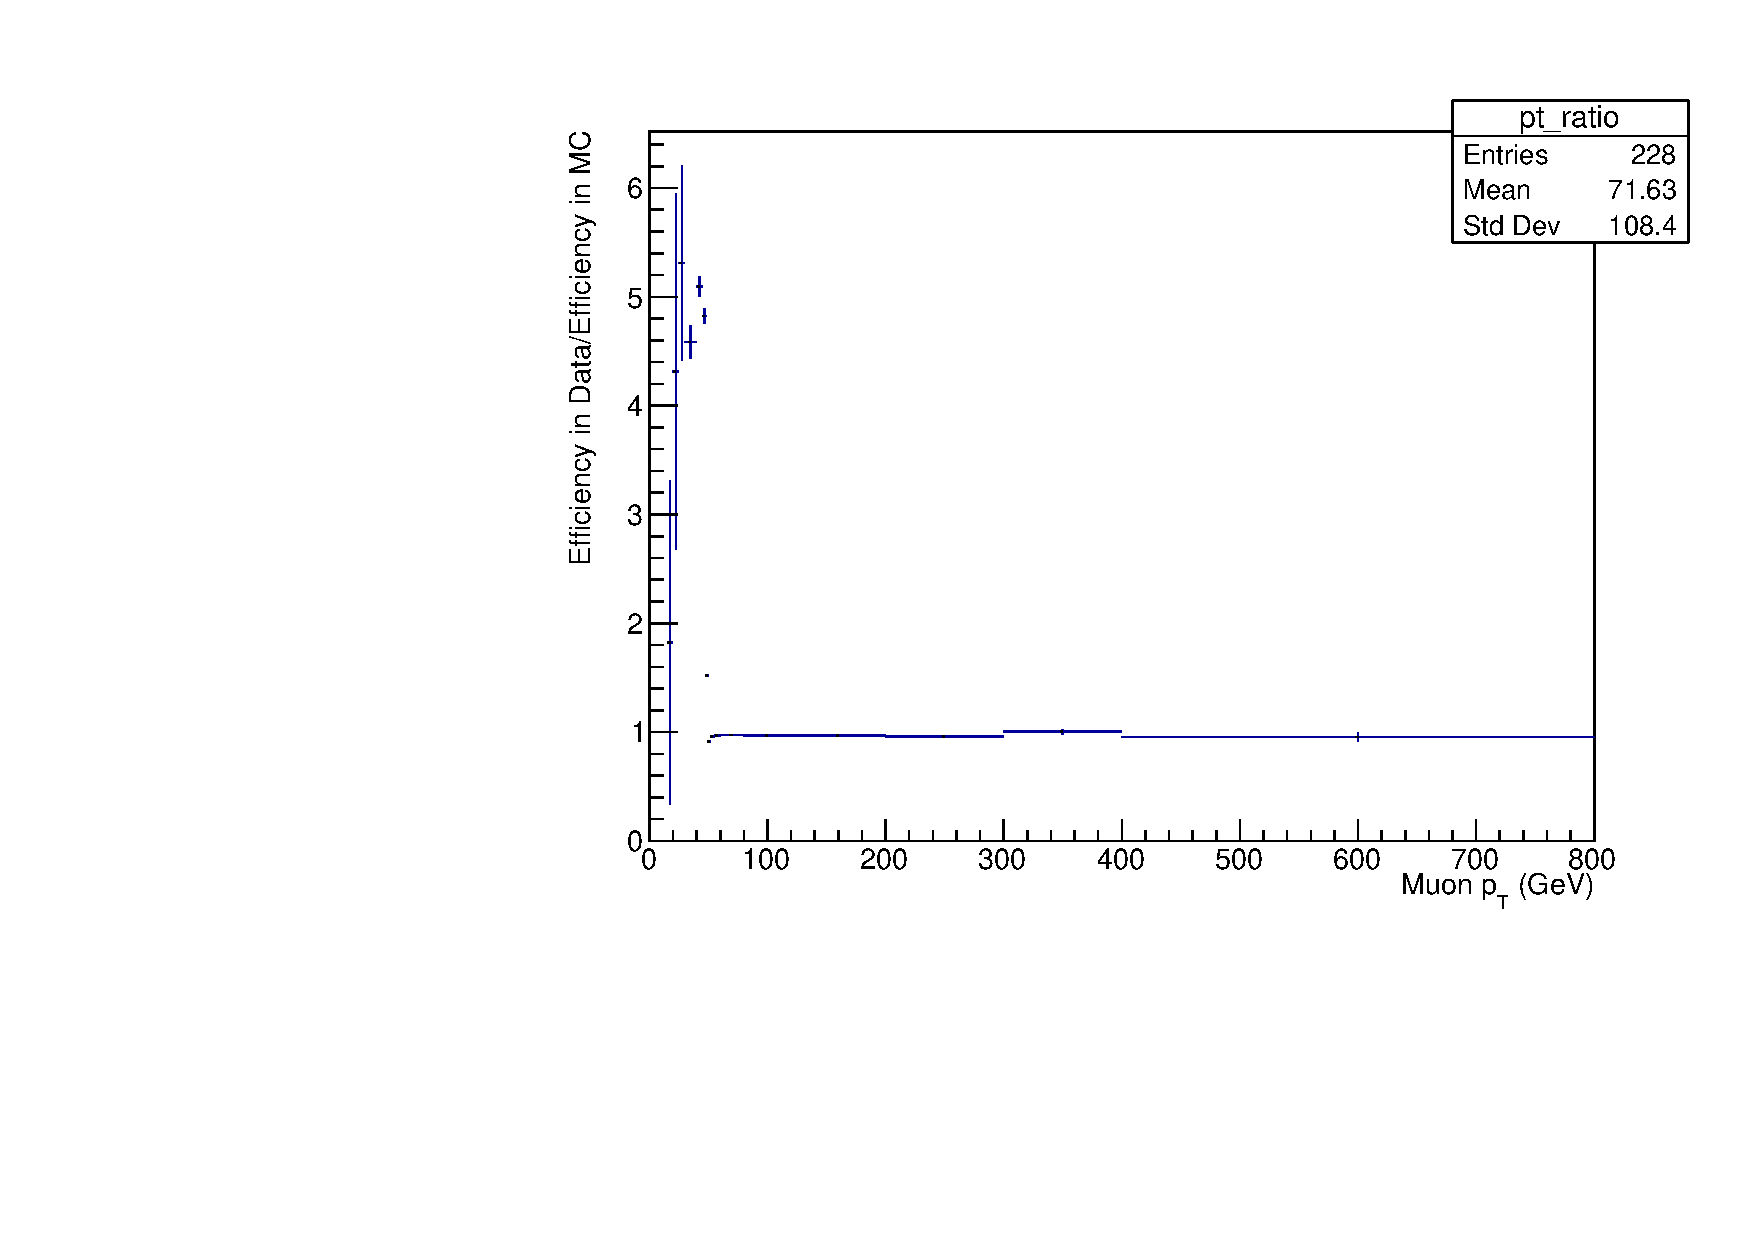
\includegraphics[width=0.49\textwidth]{figures/Run2016BtoF_MuonHLTsf.pdf}
    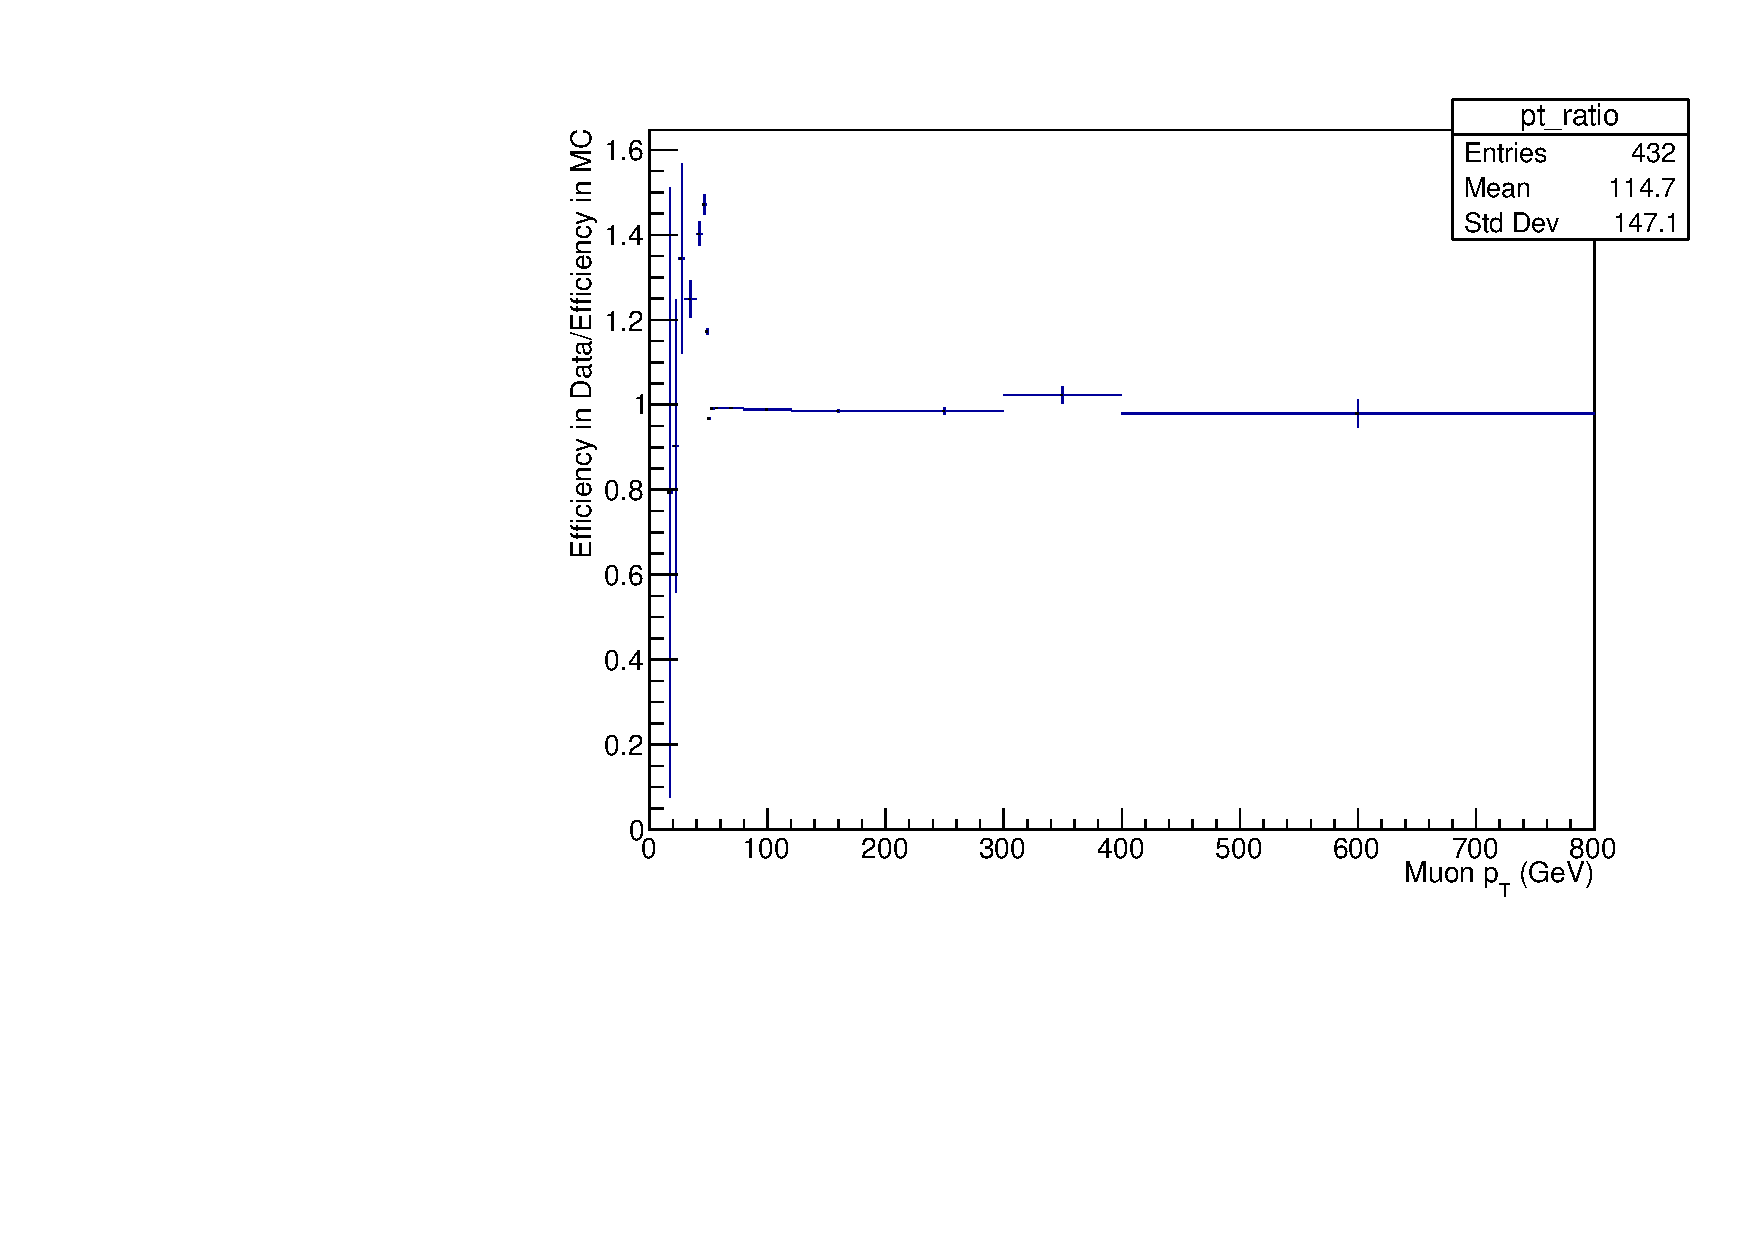
\includegraphics[width=0.49\textwidth]{figures/Run2016GtoH_MuonHLTsf.pdf}\\
    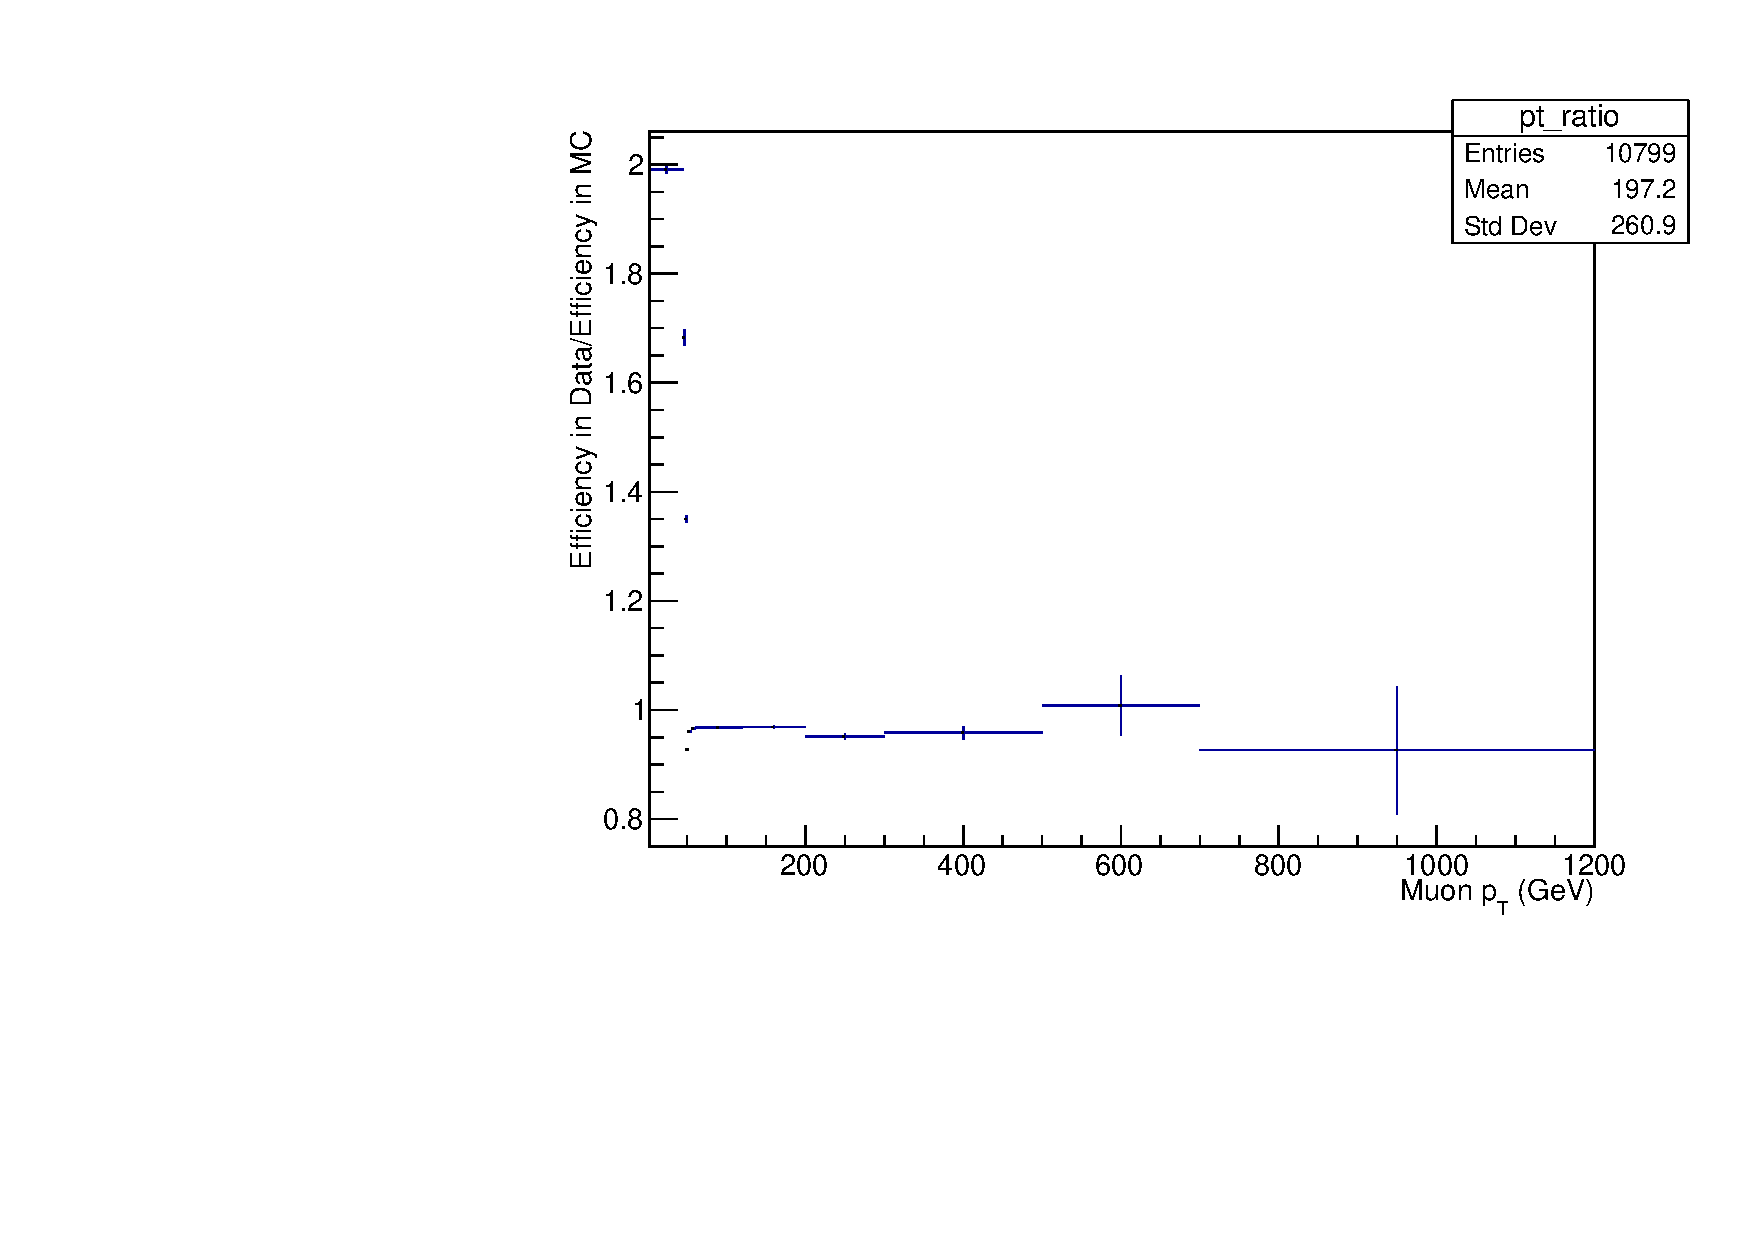
\includegraphics[width=0.49\textwidth]{figures/Run2017_MuonHLTsf.pdf}
    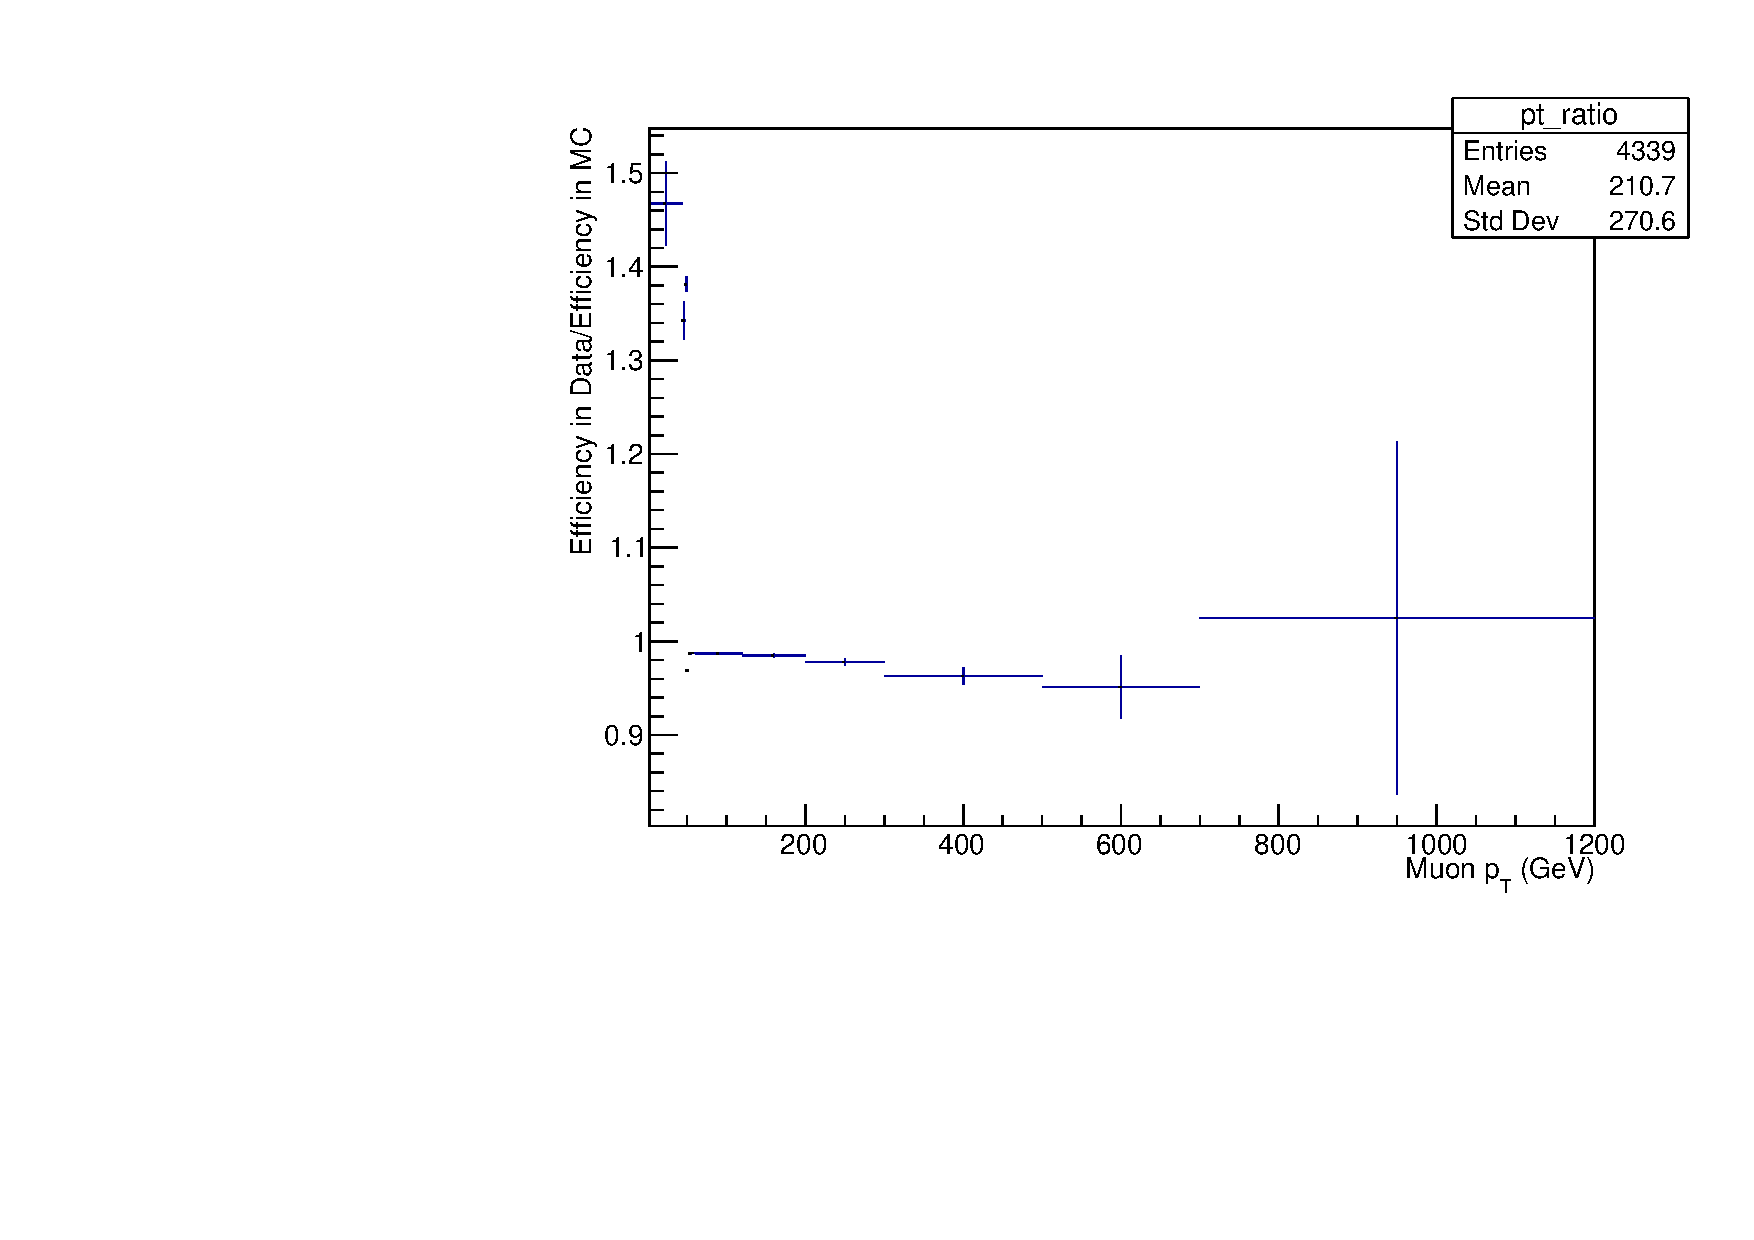
\includegraphics[width=0.49\textwidth]{figures/Run2018_MuonHLTsf.pdf}
    \caption{Muon trigger weights in Runs B-F of 2016 (top left), Runs G-H of 2016 (top right), 2017 (bottom left), and 2018 (bottom right).}
 \label{fig:MuonHLTweights}
 \end{center}
 \end{figure}

\subsection{Electron Triggers}
Electron trigger choice was more challenging than for muons. The lowest unprescaled trigger does not have perfect efficiency at higher $\pt$ where it would be expect to.  Two additional triggers were added, one higher energy electron trigger and one higher energy photon trigger.  At high energies, photon and electron identification is less efficient for the HLT, and combining these two triggers raises the efficiency.  Electrons and photons can then be later differentiated with parameters not used by the trigger.


\begin{table}[htbp]
  \caption{
    Electron Selection Triggers
  }
  \centering
  \label{tab:MuTrig}
  \begin{tabular}{l c}
    \hline
    Year & Trigger \\
    \hline
    2016 & \tt HLT\_Ele27\_WPTight\_Gsf\_v* OR HLT\_Ele115\_CaloIdVT\_GsfTrkIdT OR HLT\_Photon175\_v* \\
    2017 & \tt HLT\_Ele35\_WPTight\_Gsf\_v* OR HLT\_Ele115\_CaloIdVT\_GsfTrkIdT OR HLT\_Photon200\_v* \\
    2018 & \tt HLT\_Ele32\_WPTight\_Gsf\_v* OR HLT\_Ele115\_CaloIdVT\_GsfTrkIdT OR HLT\_Photon200\_v* \\
    \hline
  \end{tabular}
\end{table}

\subsubsection{Electron Trigger Efficiencies}

The electron trigger combinations used in this analysis had not been officially studied.  As it is impossible to guarantee that the behaviour of a trigger applied to MC and data will behave the same, all triggers, and trigger combinations, have to be studied.  The trigger efficiency of the trigger combinations was measured in data and MC and compared to produce a scale factor based on electron $\pt$ and $\eta$.  Graphs showing the comparison of data and MC in each of the years are shown in figure \ref{fig:electronHLTSF}.  As the majority of the $\eta$ dependence has to do with whether an electron lands in the barrel region or the endcap region.  These are shown in black and red respectively.

\begin{figure}[htbp]
  \centering
  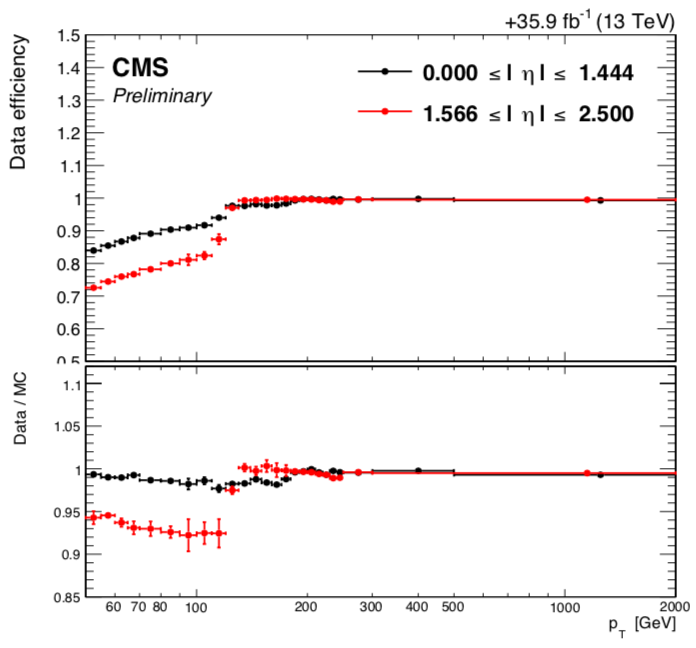
\includegraphics[width=0.45\textwidth]{figures/2016/2016_electron_HLT_SF.png}
  \vspace{0.01\textwidth}
  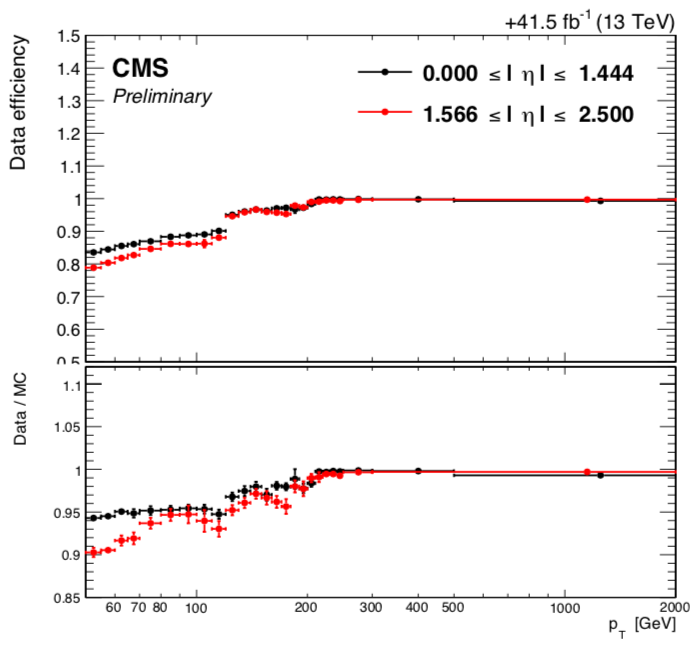
\includegraphics[width=0.45\textwidth]{figures/2017/2017_electron_HLT_SF.png}
  \vspace{0.01\textwidth}
  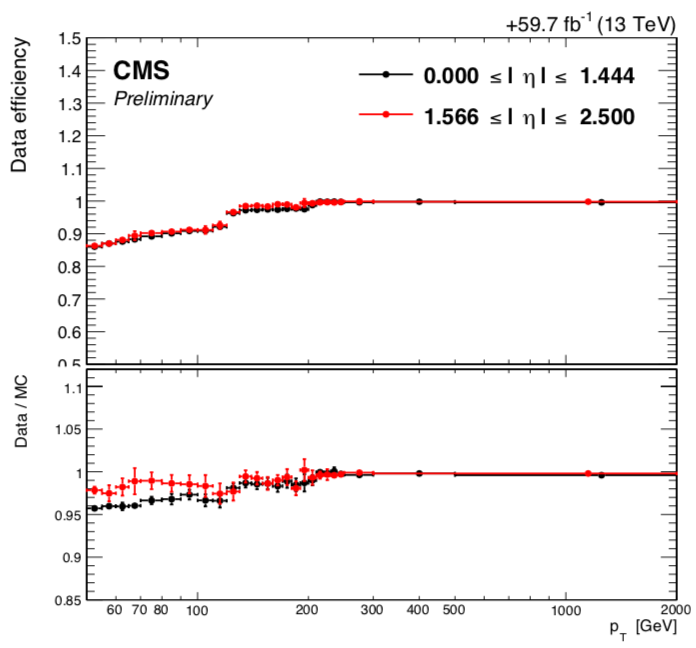
\includegraphics[width=0.45\textwidth]{figures/2018/2018_electron_HLT_SF.png}
  \caption{HLT trigger path comparison of data and MC.  Top is 2016. 2017 in the middle, and 2018 on bottom.}
 
  \label{fig:electronHLTSF}
\end{figure}

\subsubsection{Level 1 Pre-Firing Trigger Inefficiency}

An issue with the \ECAL trigger system occurred during 2016 and 2017.  Information packaged by a subdetector and sent to the level 1 (L1) trigger system are called trigger primitives.  These form the view of the \CMS detector at the L1 level.  In the inner most rings of the \ECAL endcap, the timing of the detector began to drift, which increased the L1 pre-firing rate for all of the L1 triggers based on the calorimeters.

L1 pre-firing occurs when a L1 trigger fires based on the information from a trigger primitive which does not correspond to correct bunch crossing (BX).  The trigger primitive produced by \ECAL would have come from a certain BX, but because of a timing error, the BX prior to the trigger event is actually readout and sent to the HLT.  The \CMS trigger rules, which are designed to prevent buffer overflows vetoes more than one L1 trigger acceptance (L1A) signal in three consecutive BXs. The L1A from the incorrect BX then prevents the correct BX from being readout, even if it could have passed for other reasons.
A diagram of this is shown in Figure \ref{fig:L1prefire}.
\begin{figure}[htbp]
  \centering
  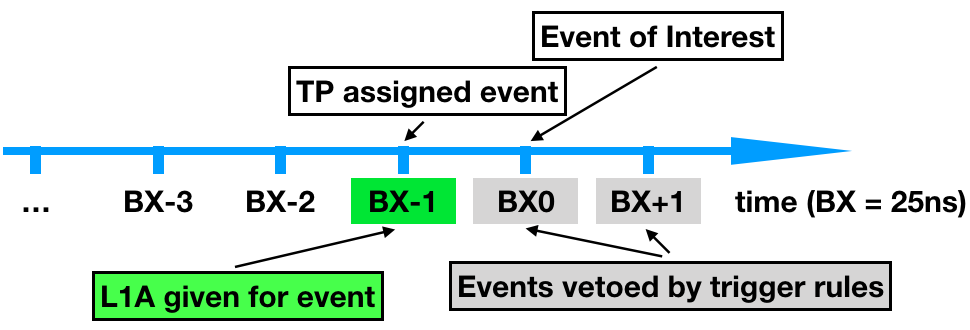
\includegraphics[width=0.45\textwidth]{figures/prefire.png}
  \caption{The event of interest is shown as BX0.  Because of the timing shift, the TP is identified as being with BX-1, the L1A is issued for the wrong event, and the next two BXs are disallowed by trigger rules}
 
  \label{fig:L1prefire}
\end{figure}
While the timing drift causing the pre-firing is understood, there is no way to know on an event-by-event level if it occurred. There is, however, a way to guarantee that pre-firing did not occur, by leveraging the trigger rules. Events with come only 3 BX after a previous L1A cannot be affected by the prefiring issue. This is shown in Figure \ref{fig:L1unprefireable}.
\begin{figure}[htbp]
  \centering
  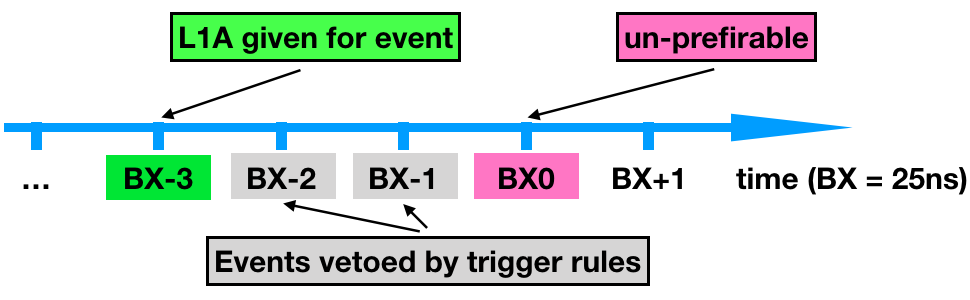
\includegraphics[width=0.45\textwidth]{figures/unprefirable.png}
  \caption{The event of interest is shown as BX0.  Because of the trigger rules, if BX-3 has an L1A generated, BX-2, and BX-1 are ignored.  This means that BX0 cannot be affected by the prefiring issue.}
 
  \label{fig:L1unprefireable}
\end{figure}

Each event that is saved records not just the L1 trigger information for the event, but also for the two BXs before and after. This means the probability that an L1 prefire could have occurred, if were not for the trigger rules, can be calculated for these unprefireable events. Using a tag-and-probe technique, the probability that an \ECAL interacting object will could have its TP energy placed in the wrong BX can be calculated.  This effect needs to studied for every analysis done using \ECAl, as each analysis will have different event requirements, changing the way the issue affects it.

The pre-firing probabilities for this analysis are measured as a function of the $\pt$ and $\eta$ for jets, which deposit significant energy in \ECAL.  The events studied must have exactly one muon which corresponds to a passing decision from the HLT IsoMu24/27.  Electrons are vetoed.  The probed jet is required to pass tight identification requirements and be isolated with $\pt > \SI{40}{\GeV}$ as well as $1.75 < \abs{\eta} < 3.5$, placing it in the endcap, where prefiring can happen.  The prefiring probabilities for this are shown in Figure \ref{fig:prefireprobs}.
\begin{figure}[htbp]
  \centering
  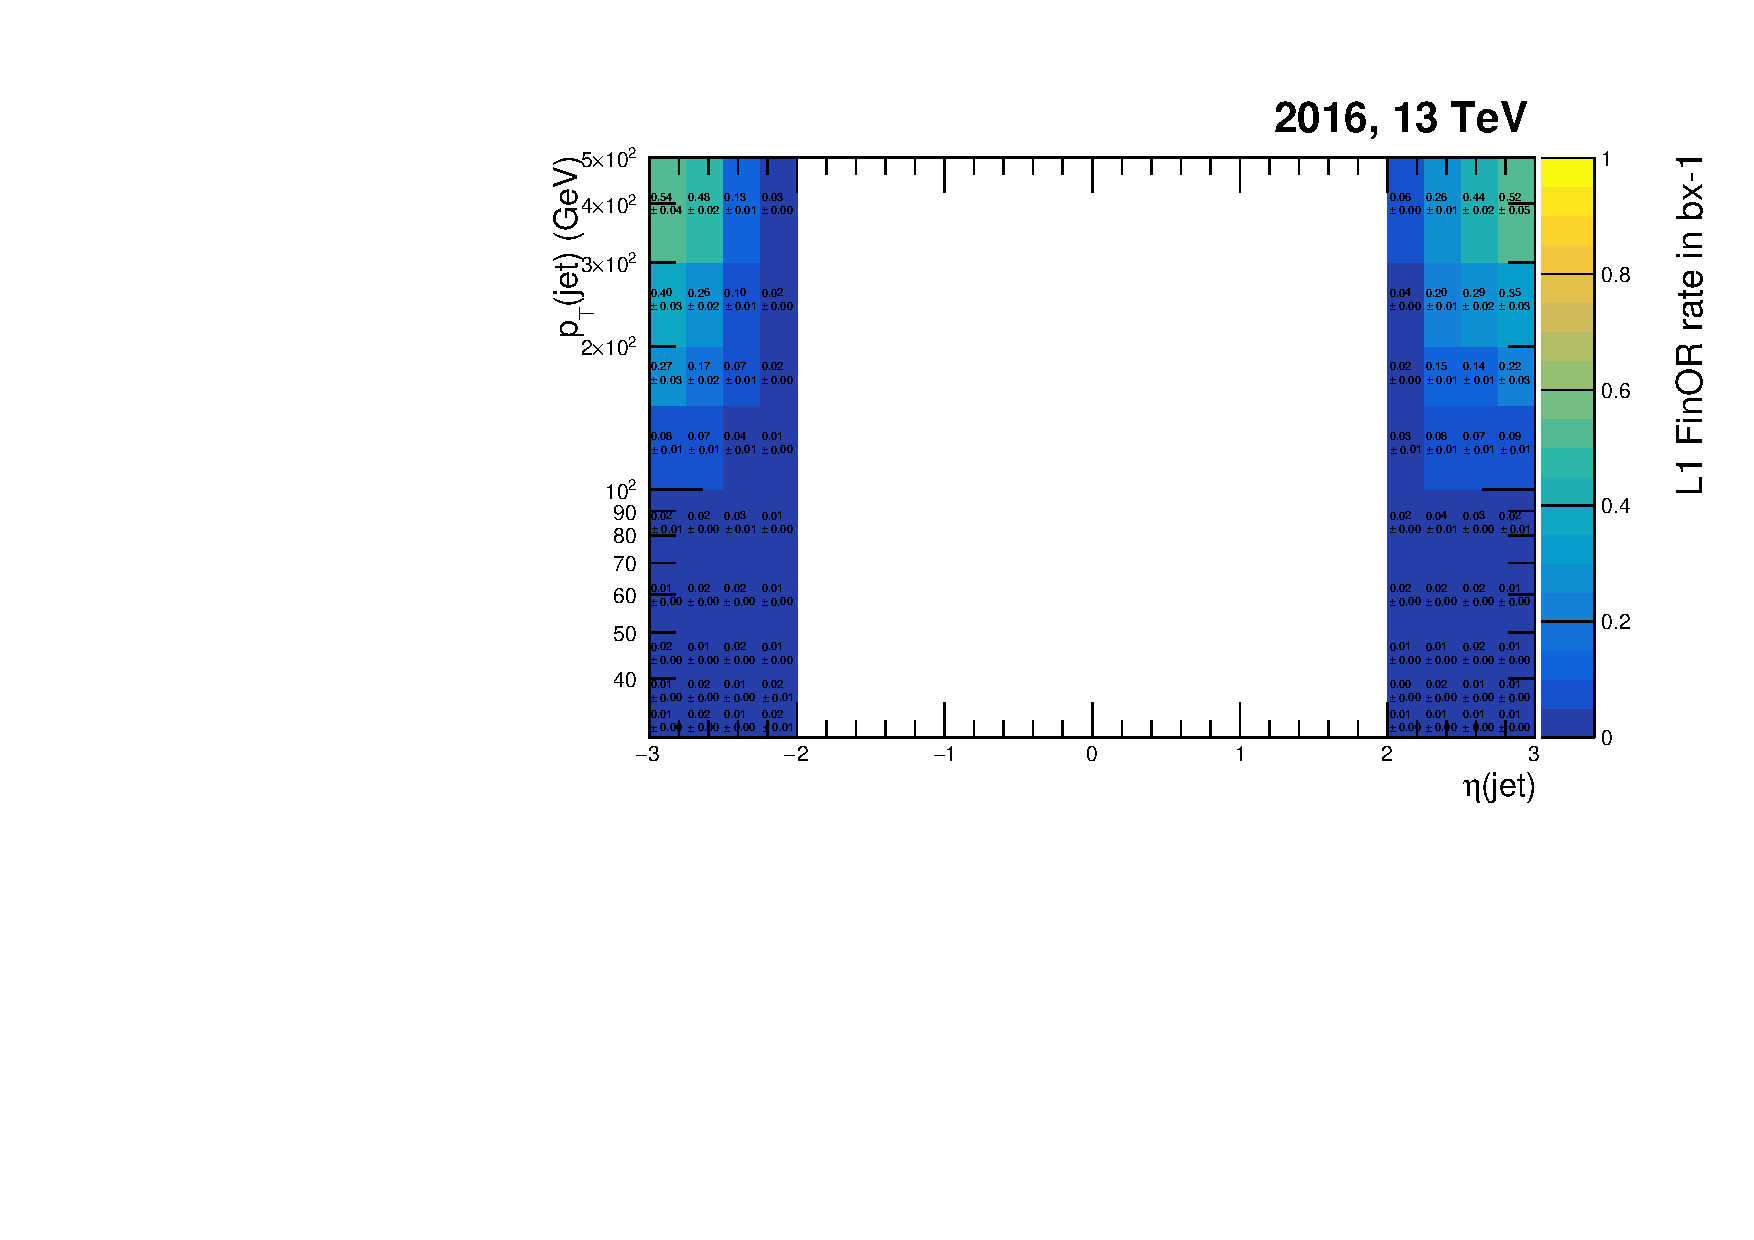
\includegraphics[width=0.45\textwidth]{figures/L1prefiring_jetpt_2016BtoH.pdf}
  \hspace{0.01\textwidth}
  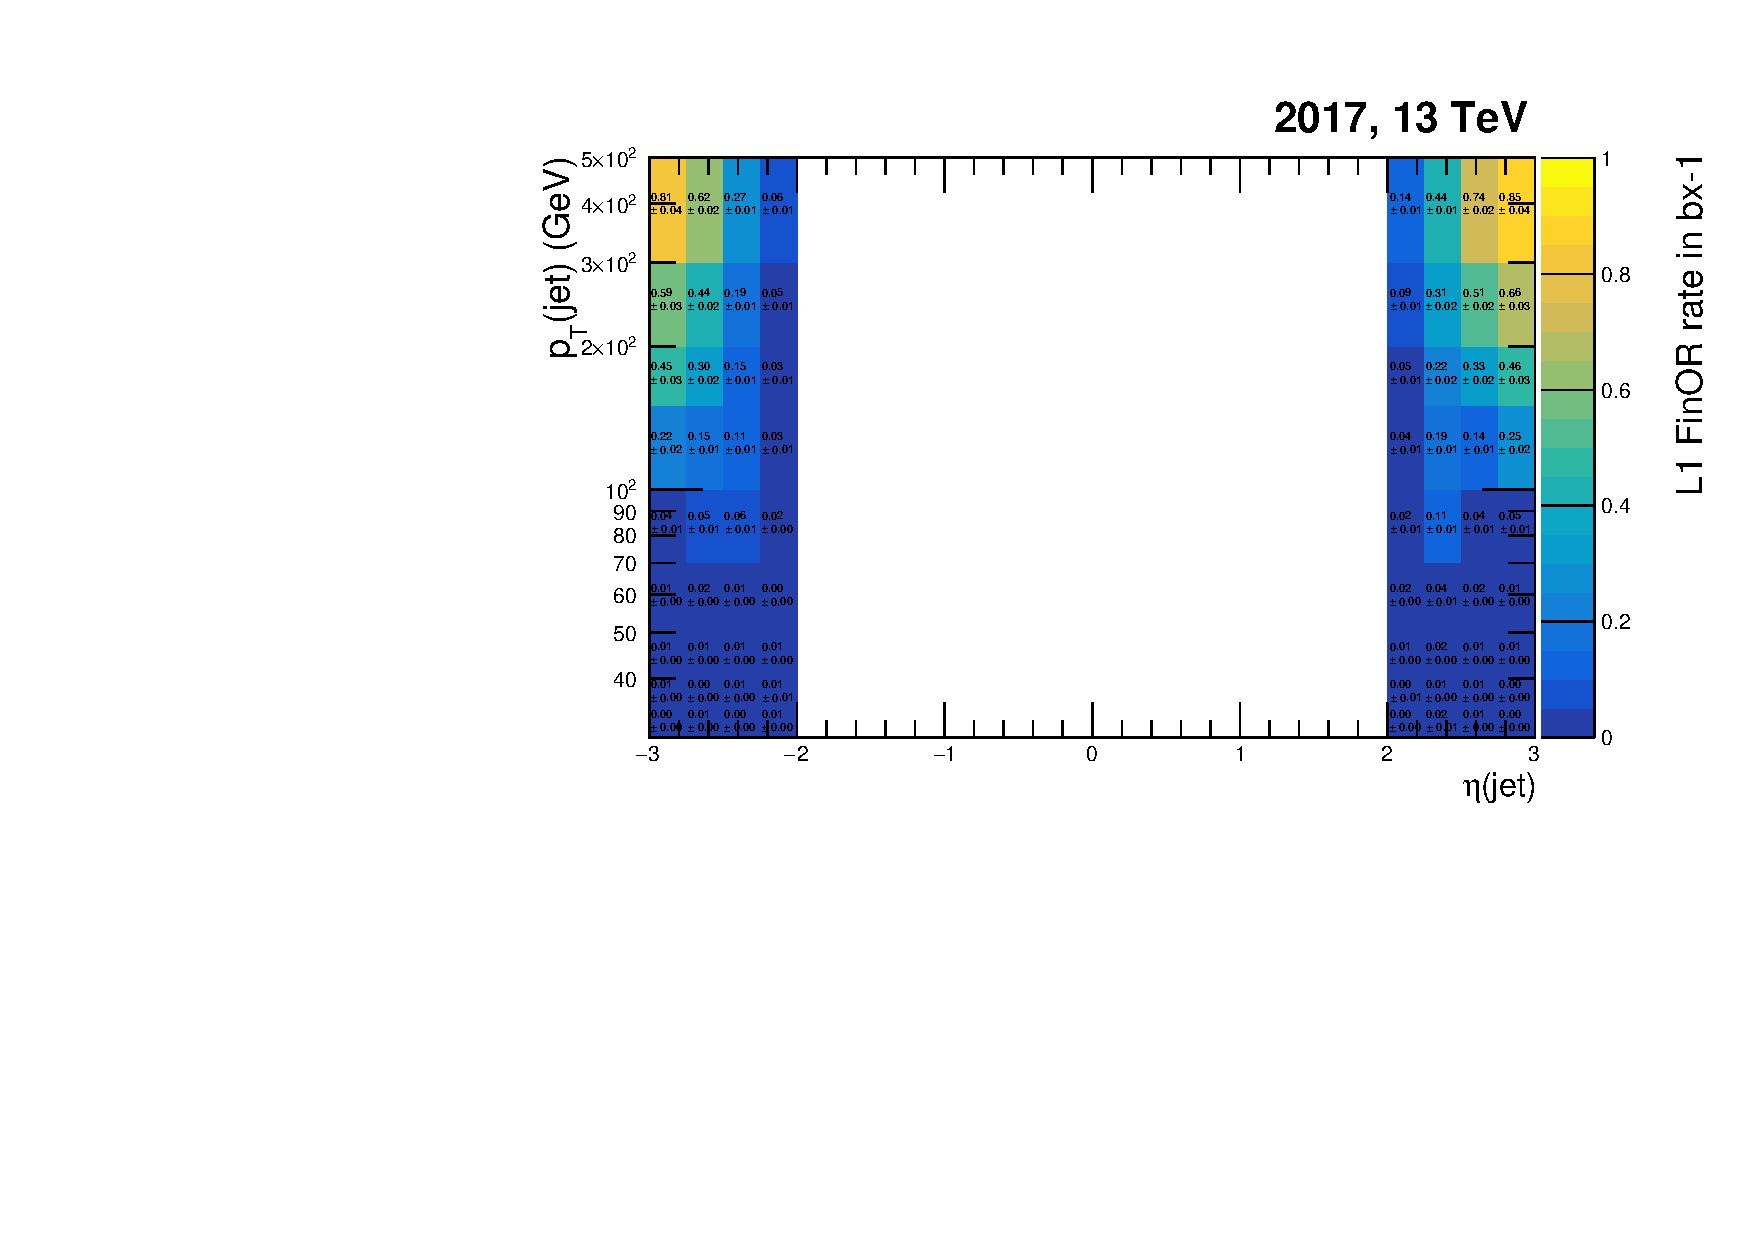
\includegraphics[width=0.45\textwidth]{figures/L1prefiring_jetpt_2017BtoF.pdf}
  \caption{The jet prefiring probability for 2016 (left) and 2017 (right).}
  \label{fig:prefireprobs}
\end{figure}

These prefiring probabilities are used to adjust the jet rate in 2016 and 2017, as simulated events do not have the prefiring issue, resulting in a mismatch of rates.

\section{Boosted Selection}

\subsection{Lepton Selection}

\subsubsection{Tight Electrons}

\subsubsection{Loose Electrons}

\subsubsection{Tight Muons}

\subsection{Event Selection}

\subsection{Jet Selection}

\subsection{Event Selections}

\subsubsection{Signal Region}

\begin{description}
\item[Boosted signal region:] \
  \begin{itemize}
  \item \textbf{$ee$ channel:} $ee$ triggers from Section~\ref{sec:triggers}.
  \item \textbf{$\mu\mu$ channel:} $\mu\mu$ triggers from Section~\ref{sec:triggers}.
  \item if 4 final state resolved objects found, then dR between the sub-leading muon and each AK4 jet $>0.4$: preserve orthogonality between boosted and resolved regions
  \item leading tight lepton with $\pt > \SI{60}{\GeV}$
  \item sub-leading loose lepton with $\pt >\SI{53}{\GeV}$
  \item at least one AK8 jet with  $\pt >\SI{200}{\GeV}$ \&\& $LSF > 0.7$ \&\& soft drop mass$ > \SI{40}{\GeV}$
  \item the sub-leading lepton must fall within the cone of the AK8 jet
  \item all leptons and jets with $|\eta| < 2.4$
  \item di-lepton mass $m_{ll} > \SI{200}{\GeV}$: to suppress DY+jets contribution
  \item $\Delta \phi > 2.0$ between selected jet and lead lepton
  \item $M_{l J} > \SI{600}{\GeV}$
  \end{itemize}
\end{description}

\subsubsection{Low $M_{lj}$ control region}

\begin{description}
\item[low $M_{lJ}$ boosted control region:]\ \\This is the control region to check our ttbar background prediction for our boosted analysis and derive a systematic uncertainty
  \begin{itemize}
  \item same as boosted signal region, but $M_{l j} < \SI{60}{\GeV}$
  \end{itemize}
\end{description}

\subsubsection{Flavor Sideband}

\begin{description}
\item[Boosted flavor sideband:]\ \\  This is the control region used to estimate the \ttbar contribution.
  \begin{itemize}
  \item \textbf{$ee$ channel} same as boosted $\mu\mu$ signal region but 1 leading muon and 1 secondary electron
  \item \textbf{$\mu\mu$ channel} same as boosted $ee$ signal region but 1 leading electron and 1 secondary muon
  \end{itemize}
\end{description}

\subsubsection{Z-mass Sideband}

\begin{description}
\item[low $M_{ll}$ boosted control region:]\ \\ This is the control region to check the agreement between data and simulation on the DY contribution.
  \begin{itemize}
  \item same as boosted signal region, but
  \item di-lepton mass $m_{ll} < \SI{150}{\GeV}$
  \item no LSF requirement on AK8 jet
  \item no requirement that sub-leading lepton be contained within the AK8 jet
  \end{itemize}
\end{description}

\section{Resolved Selection}

\subsection{Lepton Selection}

\subsection{Jet Selection}

\subsection{Event Selections}

\subsubsection{Signal Region}

\begin{description}
\item[Resolved signal region:] \
  \begin{itemize}
  \item \textbf{$ee$ channel:} $ee$ triggers from Section~\ref{sec:triggers}.
  \item \textbf{$\mu\mu$ channel:} $\mu\mu$ triggers from Section~\ref{sec:triggers}.
  \item leading tight lepton with $\pt > \SI{60}{\GeV}$
  \item sub-leading tight lepton with $\pt > \SI{53}{\GeV}$
  \item at least two AK4 jets with  $\pt > \SI{40}{\GeV}$
  \item all leptons and jets with $|\eta| < 2.4$
  \item di-lepton mass $m_{ll} > \SI{200} {\GeV}$: to suppress DY+jets contribution
  \item all objects $\Delta R > 0.4$ apart
  \item $M_{l l j j} > \SI{600}{\GeV}$
  \end{itemize}

\end{description}
\subsubsection{Low $M_{lljj}$ control region}

\begin{description}
\item[low $M_{lljj}$ resolved control region:]\ \\ This is the control region to check our ttbar background prediction for our resolved analysis and derive a systematic uncertainty
  \begin{itemize}
  \item same as resolved signal region, but $M_{l l j j} < \SI{600}{\GeV}$
  \end{itemize}
\end{description}

\subsubsection{Flavor Sideband}

\begin{description}
\item[Resolved flavor sideband:]\ \\  This is the control region used to estimate the \ttbar contribution.
  \begin{itemize}
  \item same as resolved $\mu\mu$ signal region but 1 leading electron and 1 sub-leading muon
  \end{itemize}
\end{description}

\subsubsection{Z-mass Sideband}

\begin{description}
\item[low $M_{ll}$ resolved control region:]\ \\ This is the control region to check the agreement between data and simulation on the DY contribution.
  \begin{itemize}
  \item same as resolved signal region, but
  \item di-lepton mass $m_{ll} < \SI{150}{\GeV}$
  \end{itemize}
\end{description}

\begin{figure}[htbp]
  \centering

  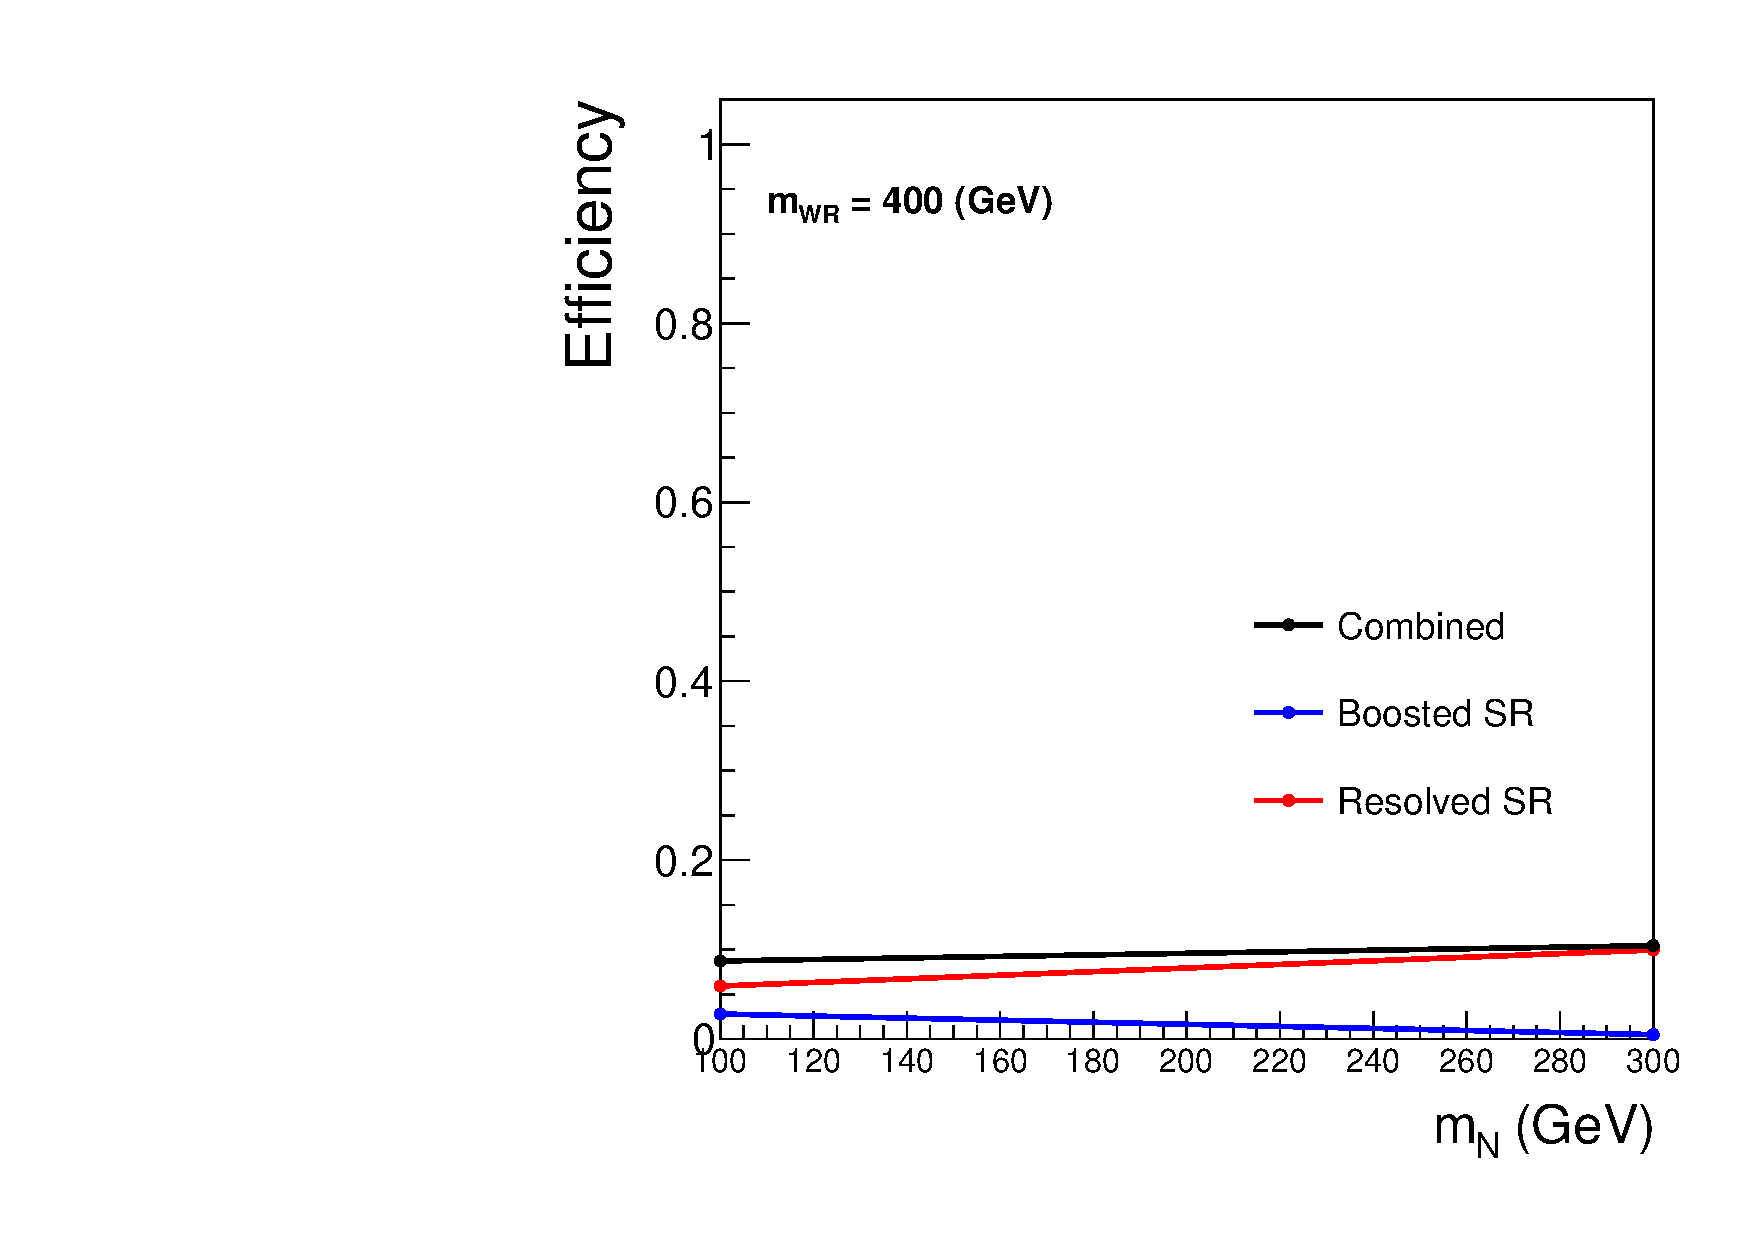
\includegraphics[width=0.45\textwidth]{figures/SigEff/WR400.pdf}
  \hspace{0.01\textwidth}
  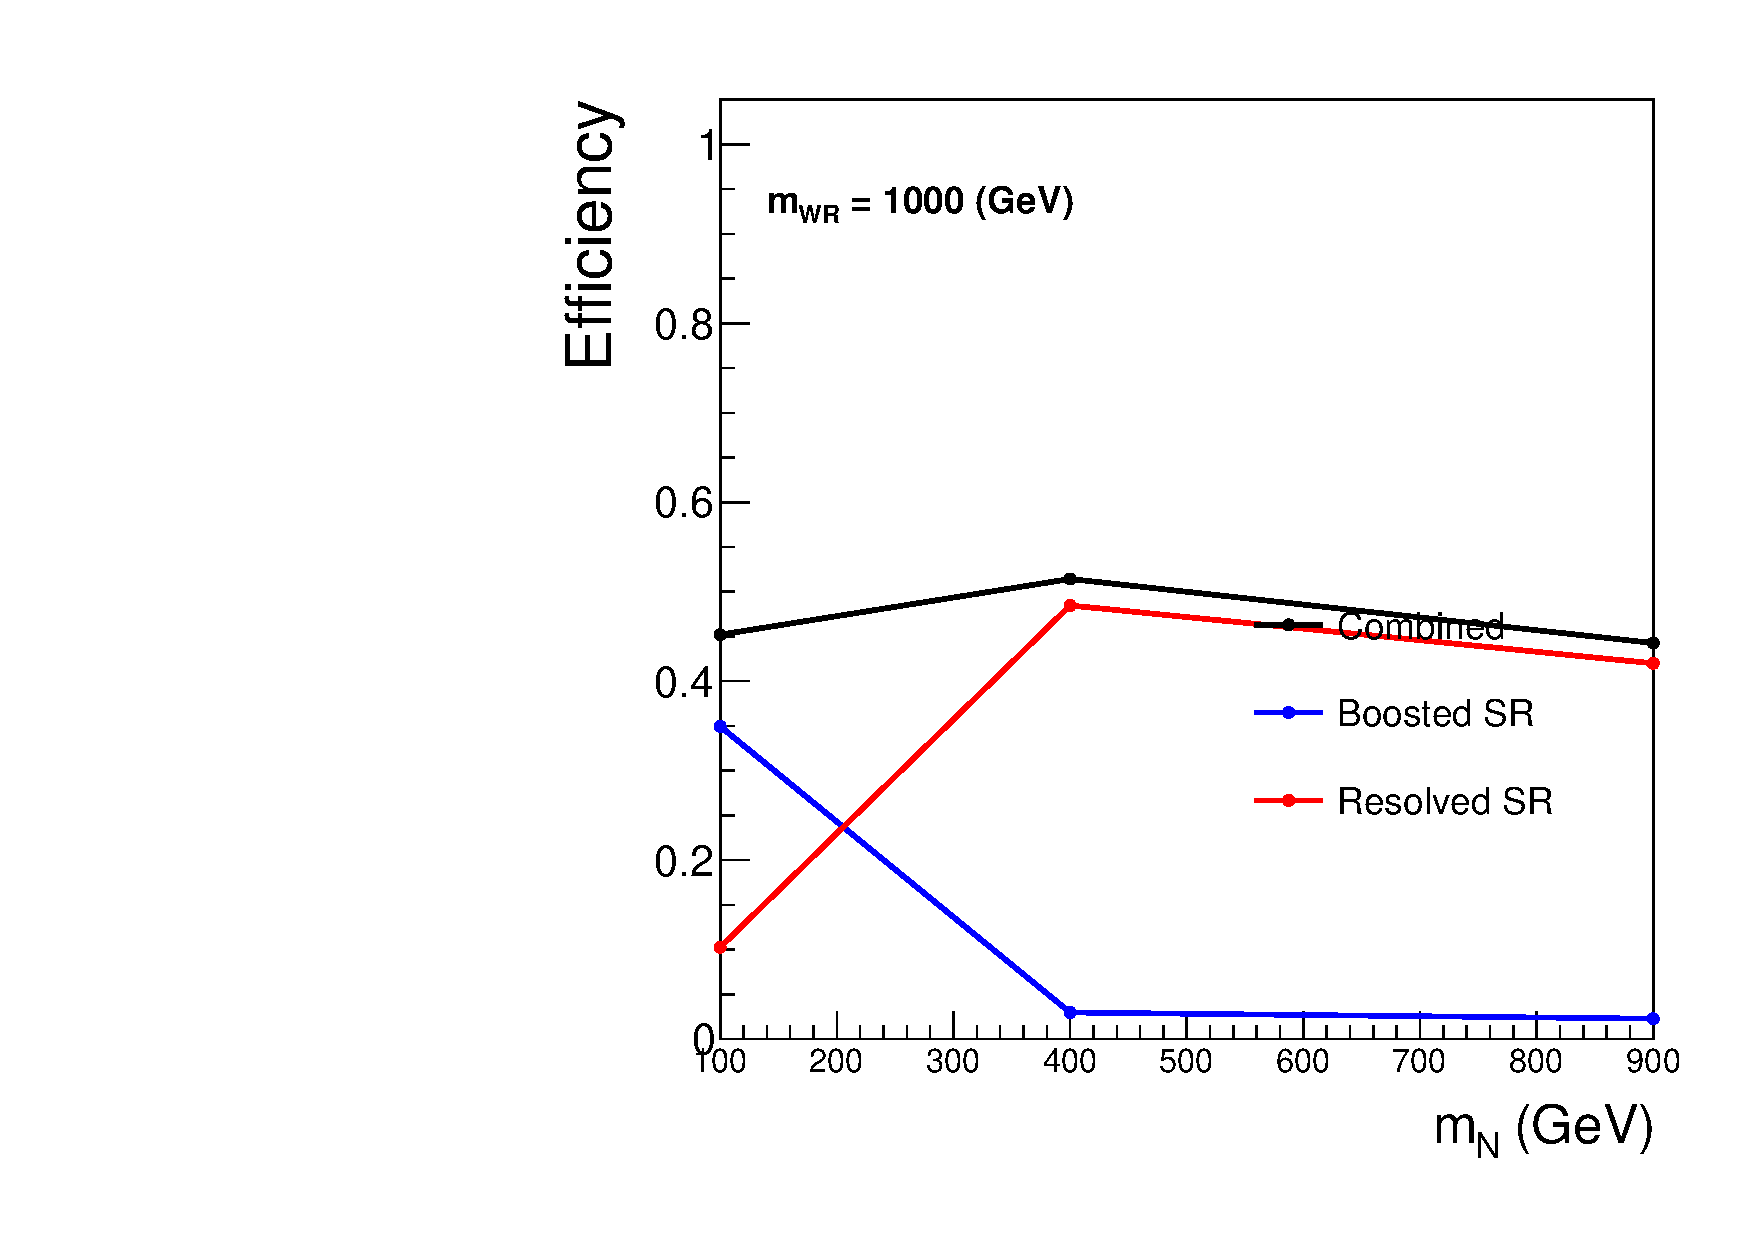
\includegraphics[width=0.45\textwidth]{figures/SigEff/WR1000.pdf}
  \vspace{0.01\textwidth}

  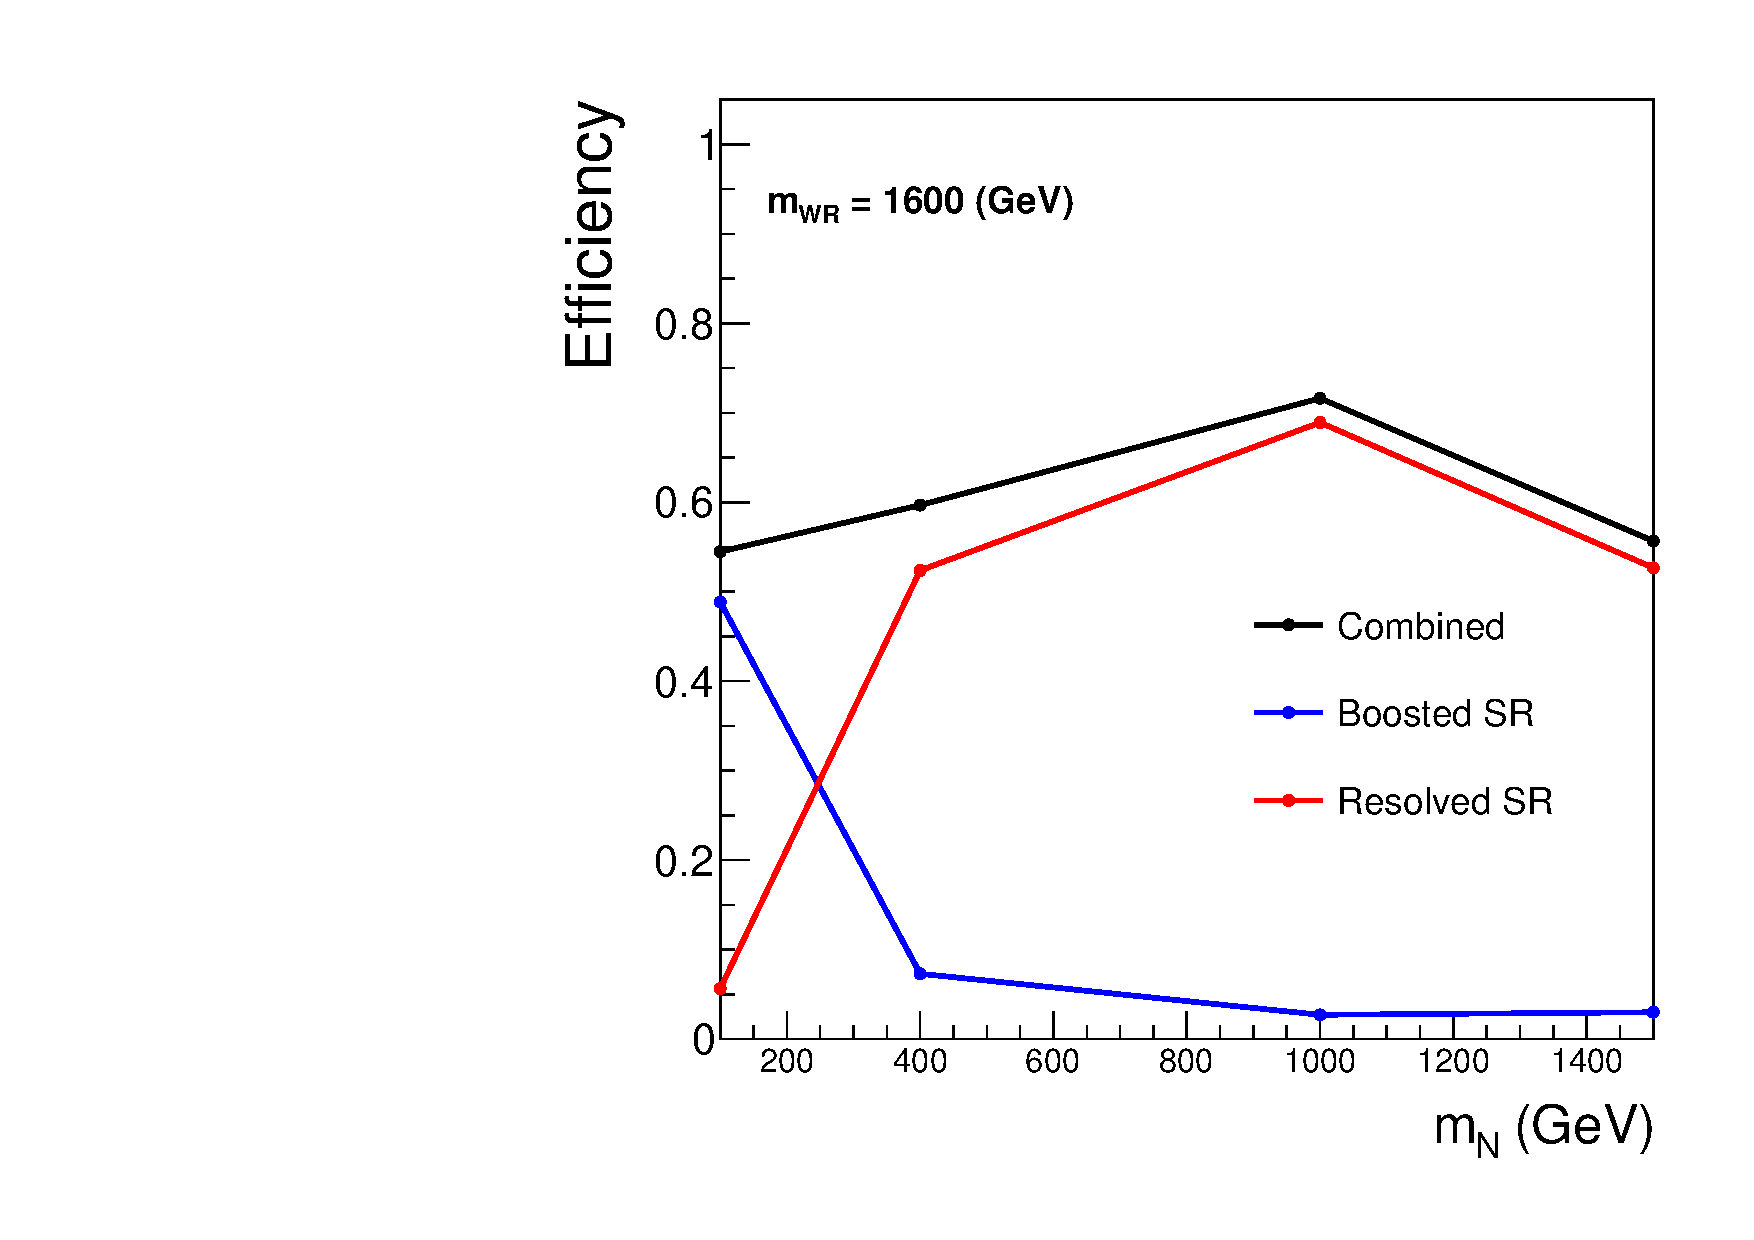
\includegraphics[width=0.45\textwidth]{figures/SigEff/WR1600.pdf}
  \hspace{0.01\textwidth}
  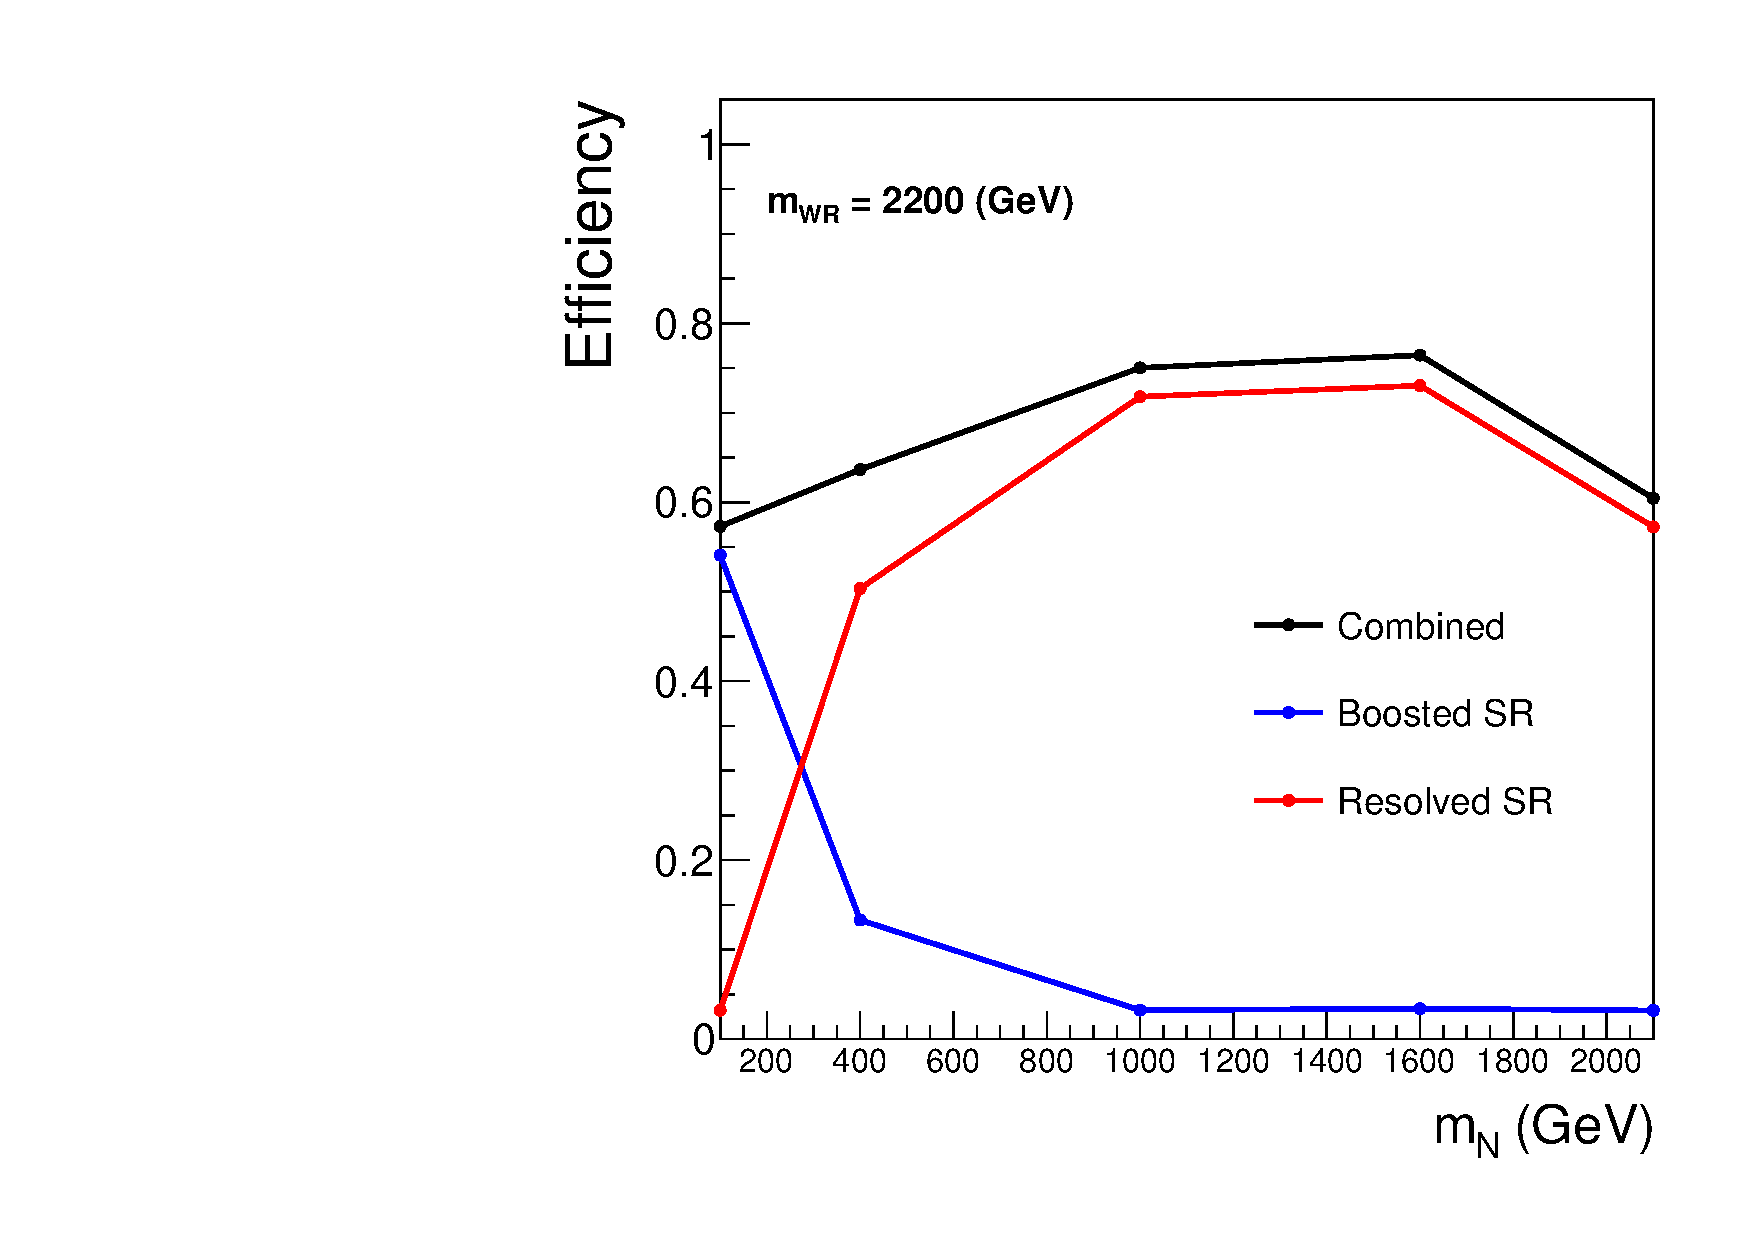
\includegraphics[width=0.45\textwidth]{figures/SigEff/WR2200.pdf}
  \vspace{0.01\textwidth}

  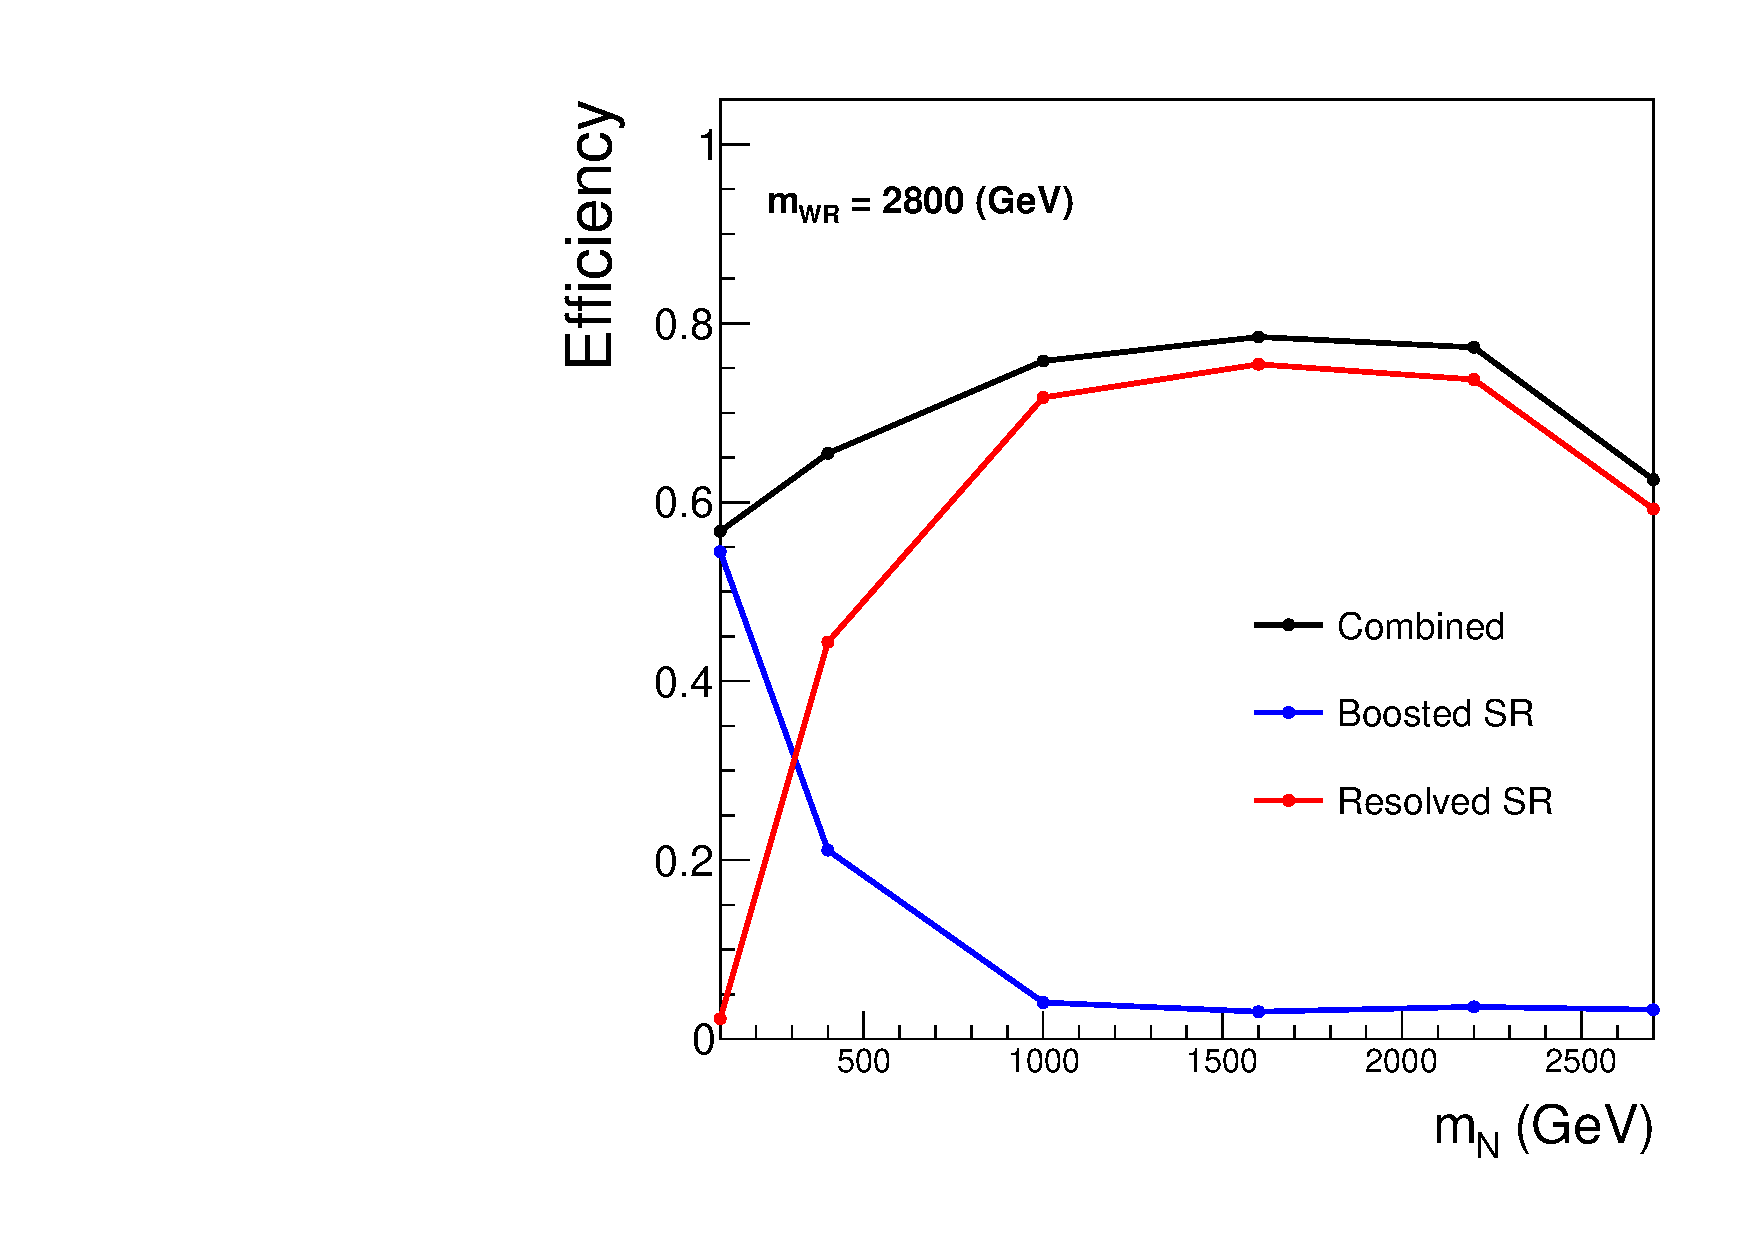
\includegraphics[width=0.45\textwidth]{figures/SigEff/WR2800.pdf}
  \hspace{0.01\textwidth}
  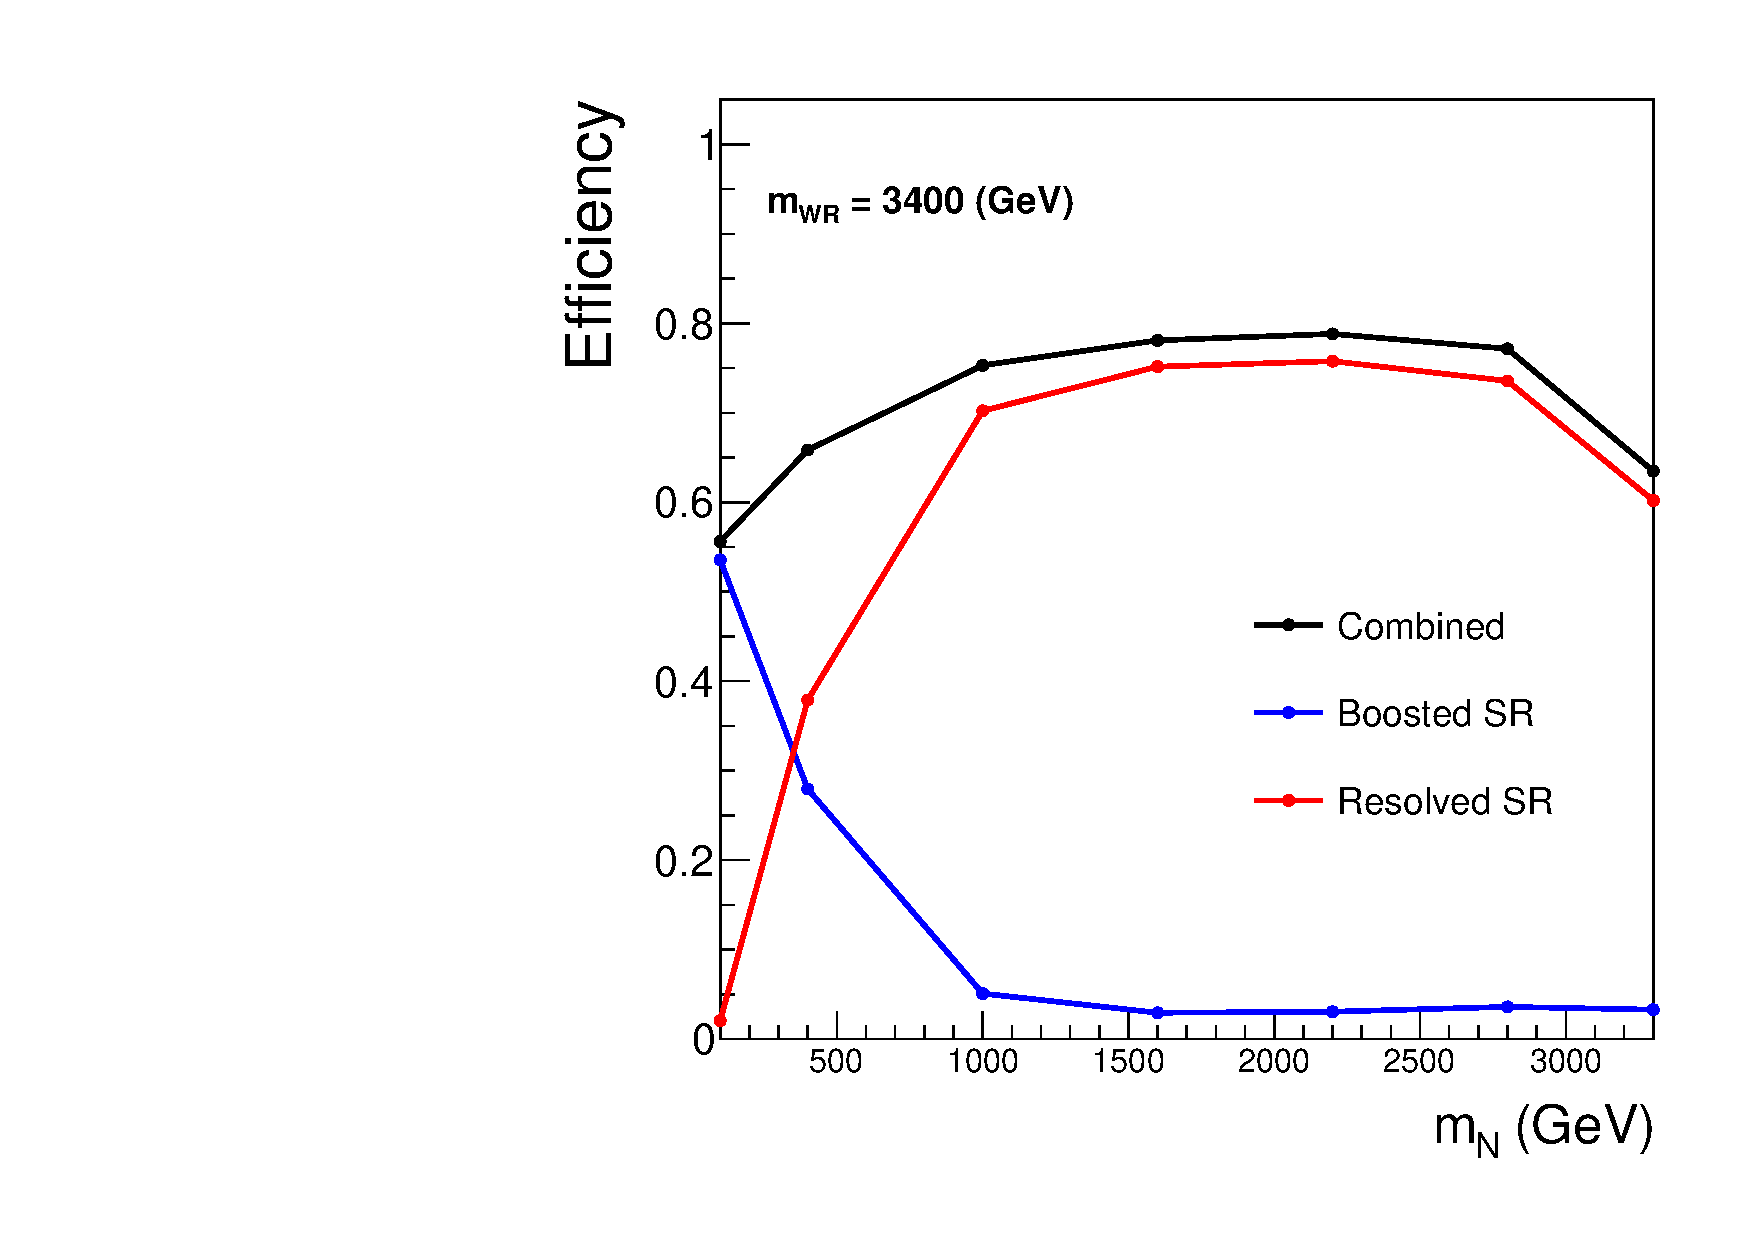
\includegraphics[width=0.45\textwidth]{figures/SigEff/WR3400.pdf}

  \caption{
    The signal efficiencies at the signal regions.
  }
  \label{fig:SigEff1}
\end{figure}

\begin{figure}[htbp]
  \centering

  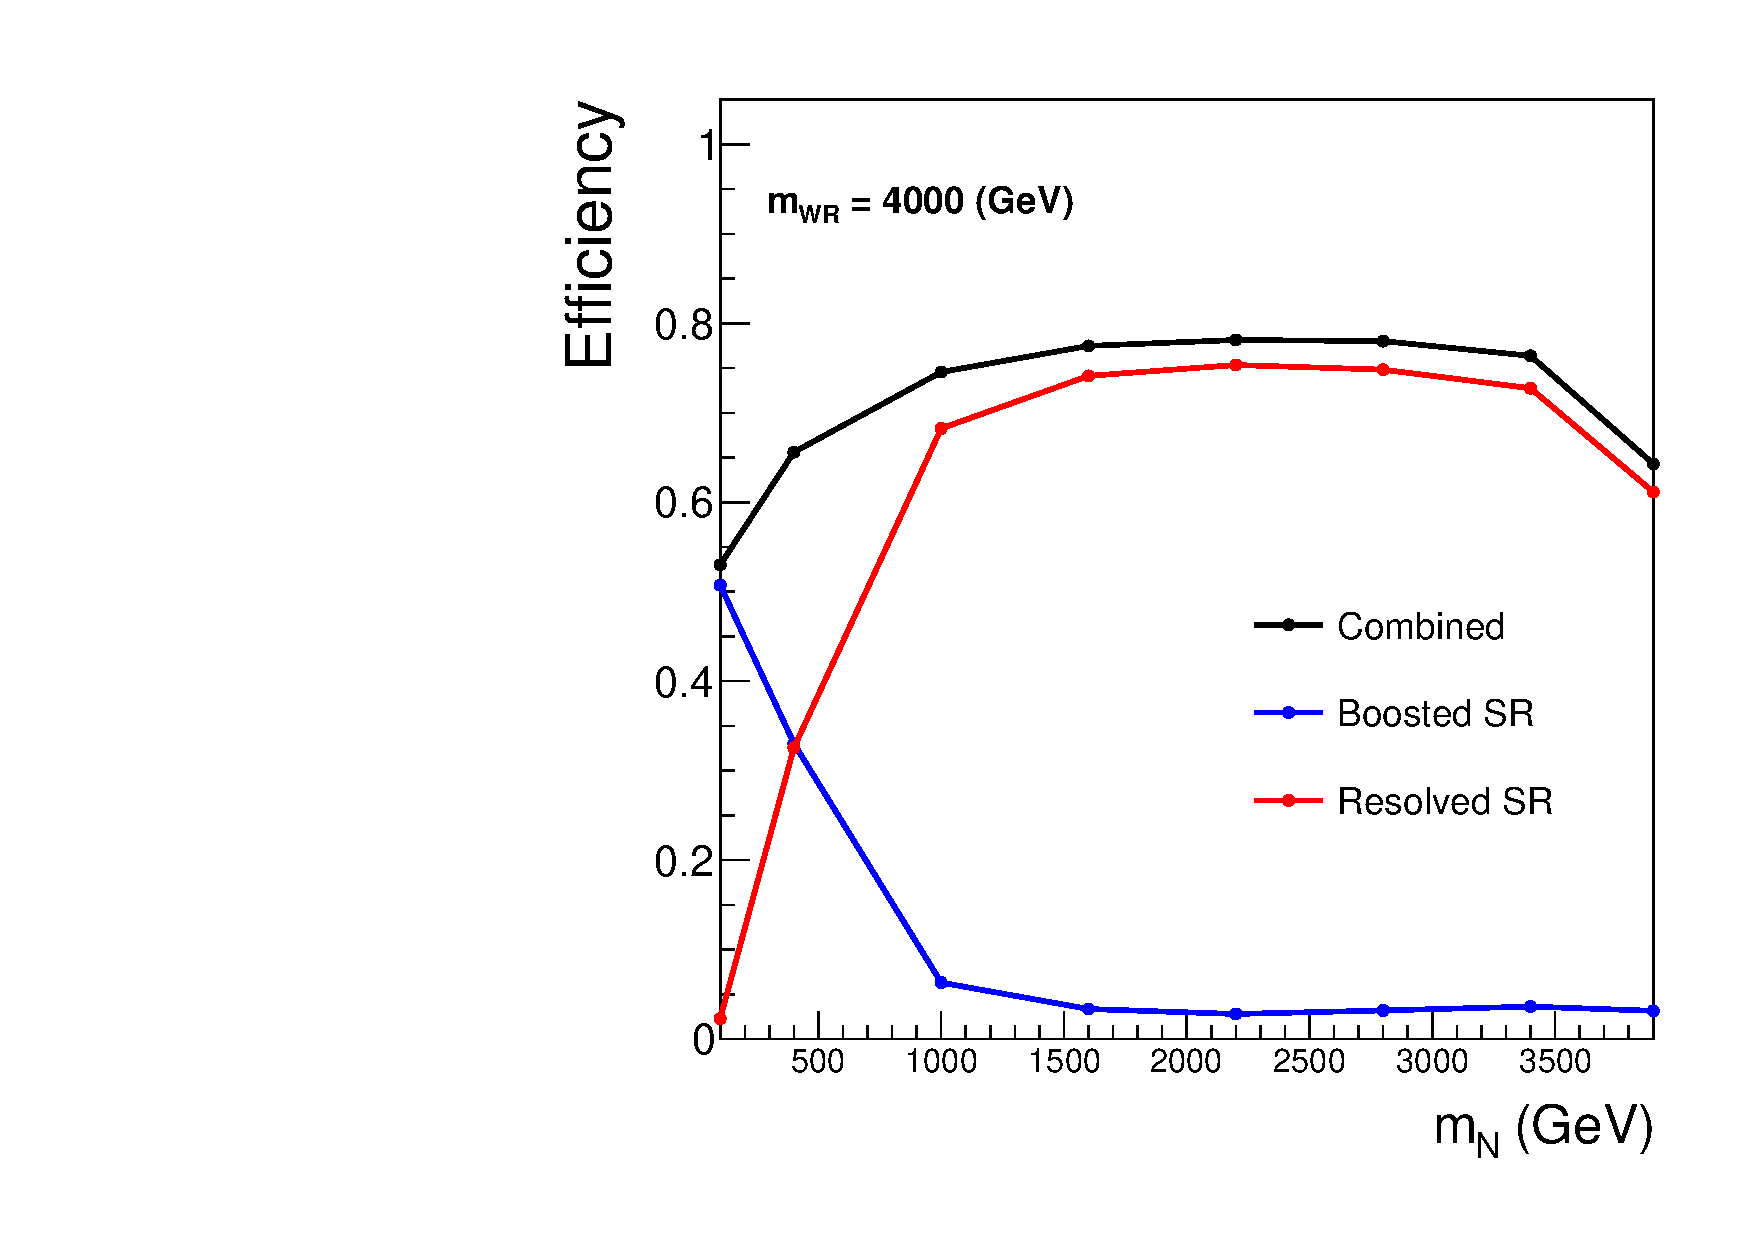
\includegraphics[width=0.45\textwidth]{figures/SigEff/WR4000.pdf}
  \hspace{0.01\textwidth}
  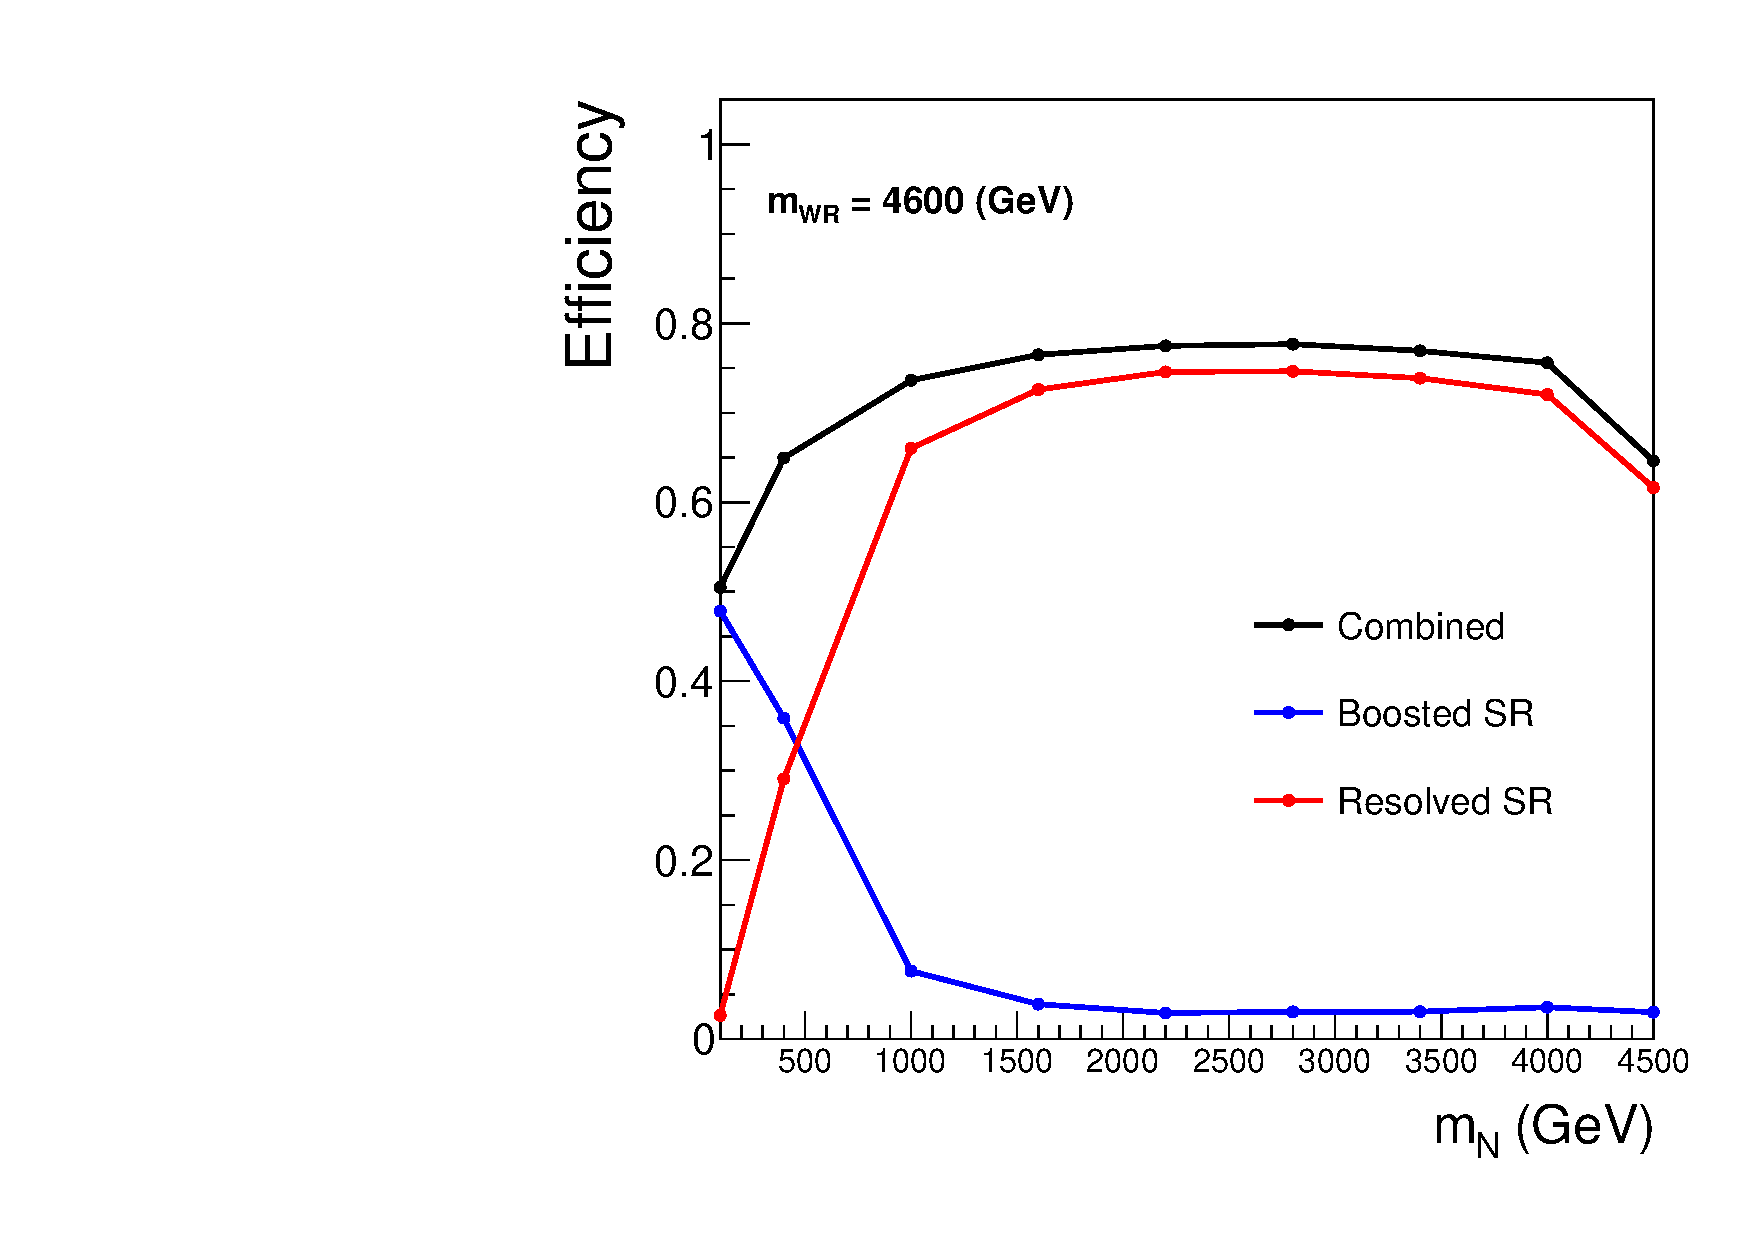
\includegraphics[width=0.45\textwidth]{figures/SigEff/WR4600.pdf}
  \vspace{0.01\textwidth}

  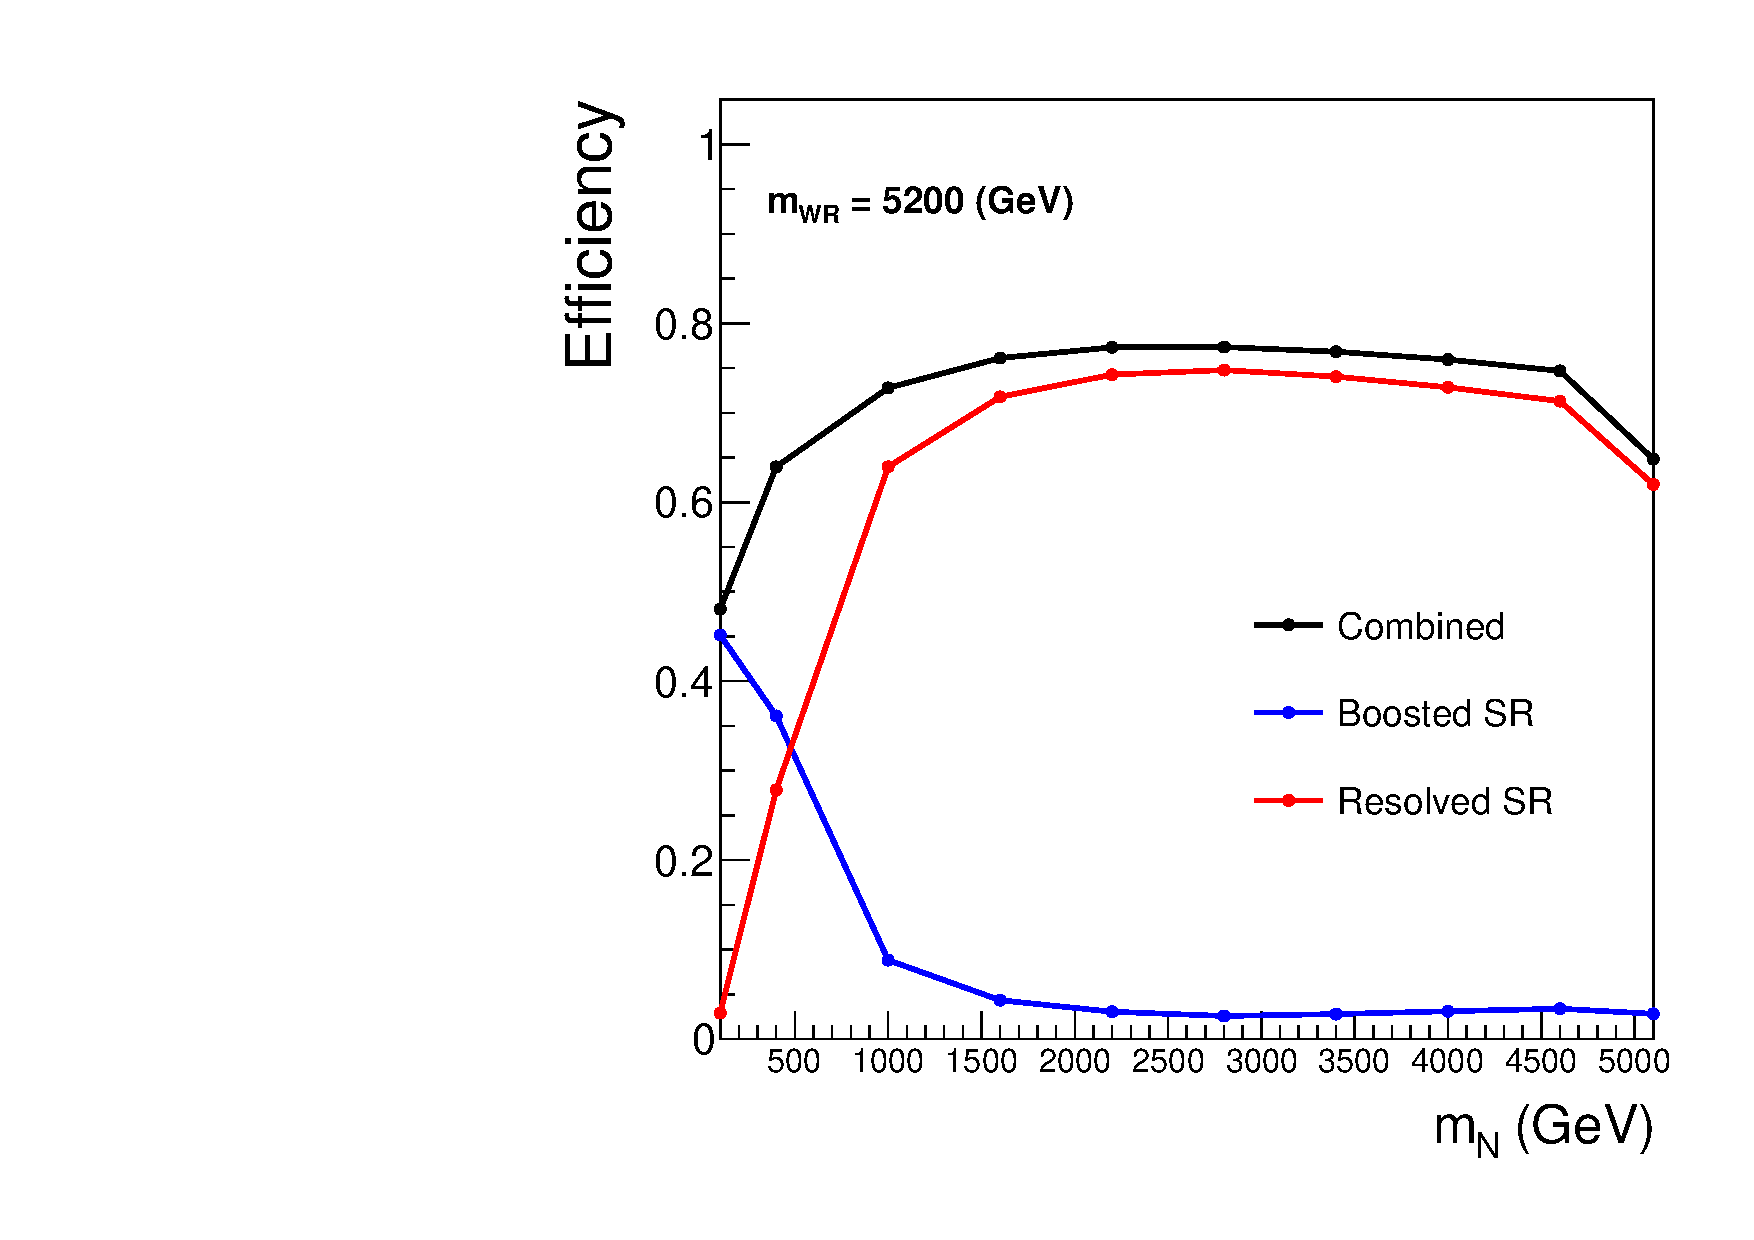
\includegraphics[width=0.45\textwidth]{figures/SigEff/WR5200.pdf}
  \hspace{0.01\textwidth}
  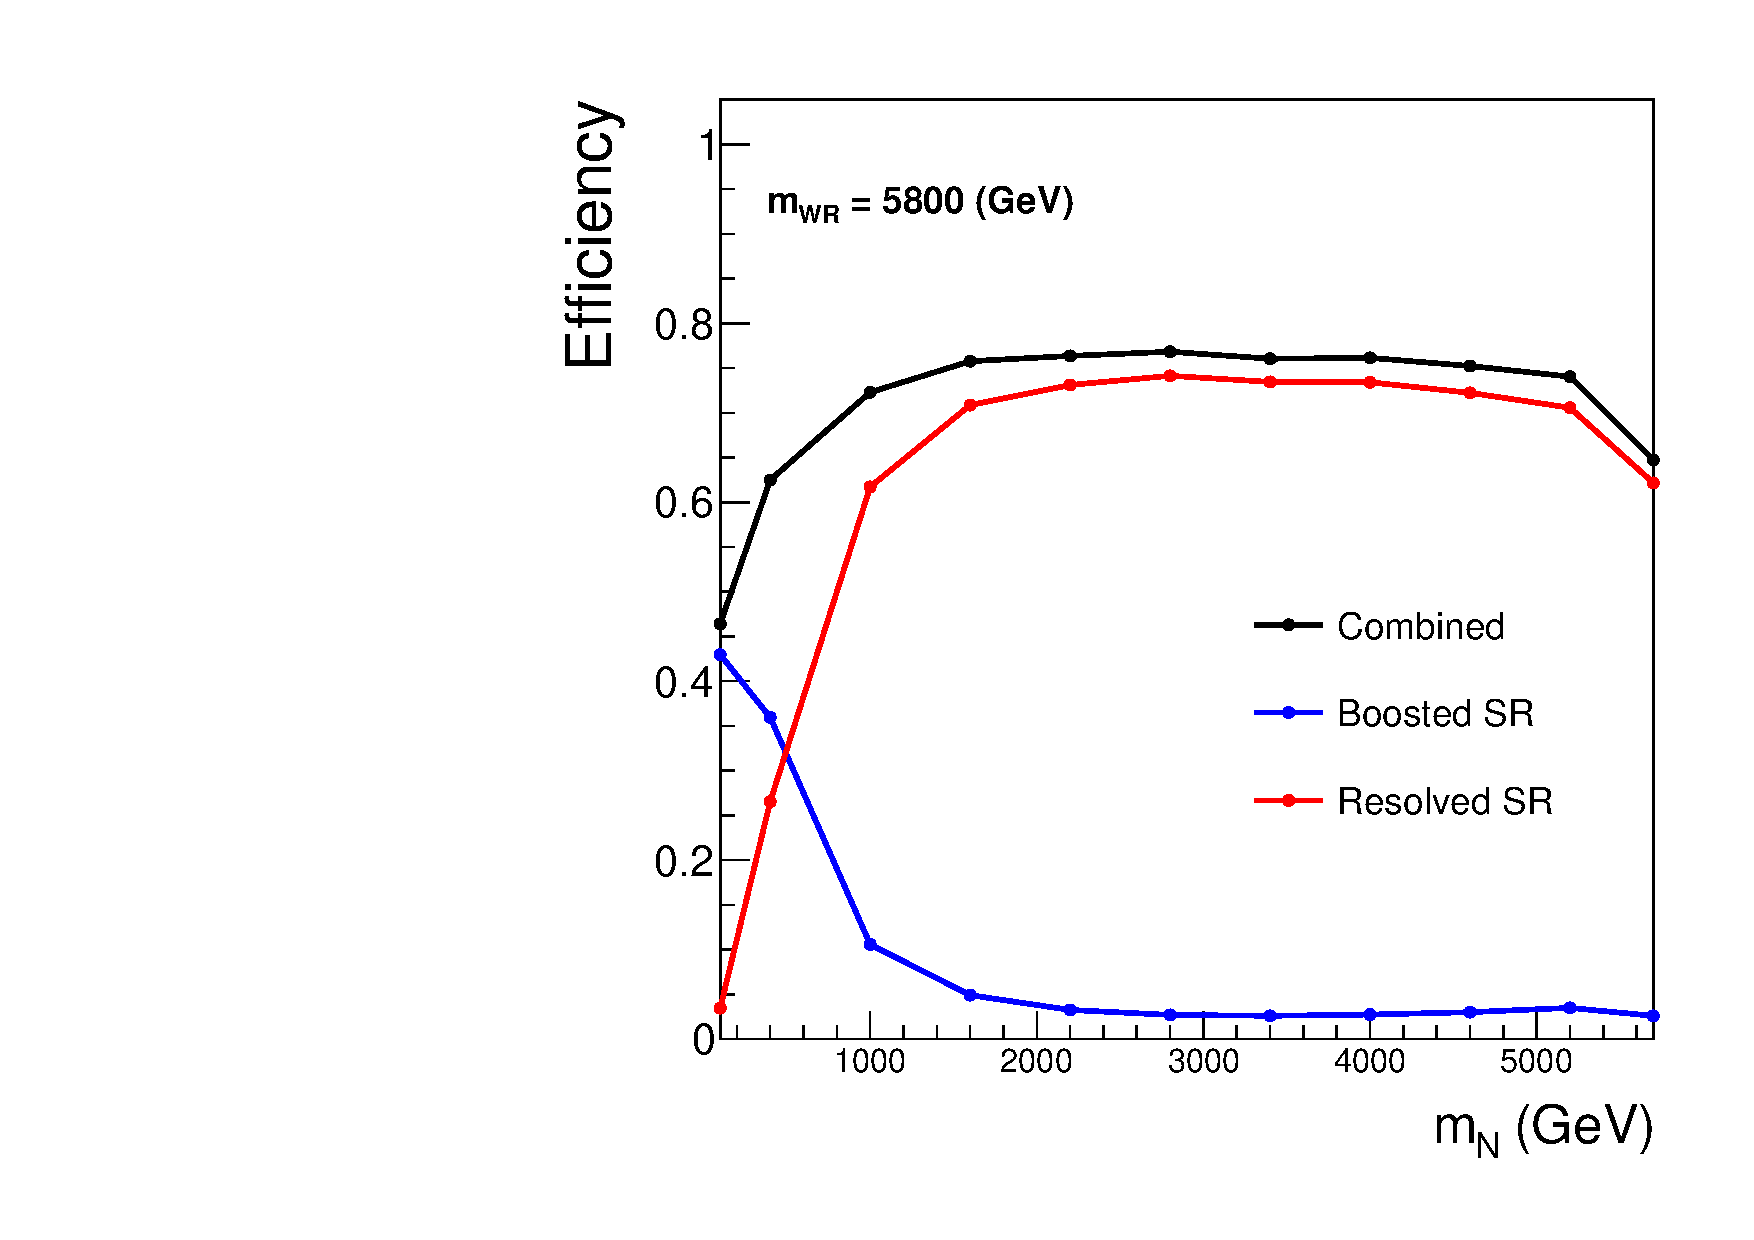
\includegraphics[width=0.45\textwidth]{figures/SigEff/WR5800.pdf}
  \vspace{0.01\textwidth}

  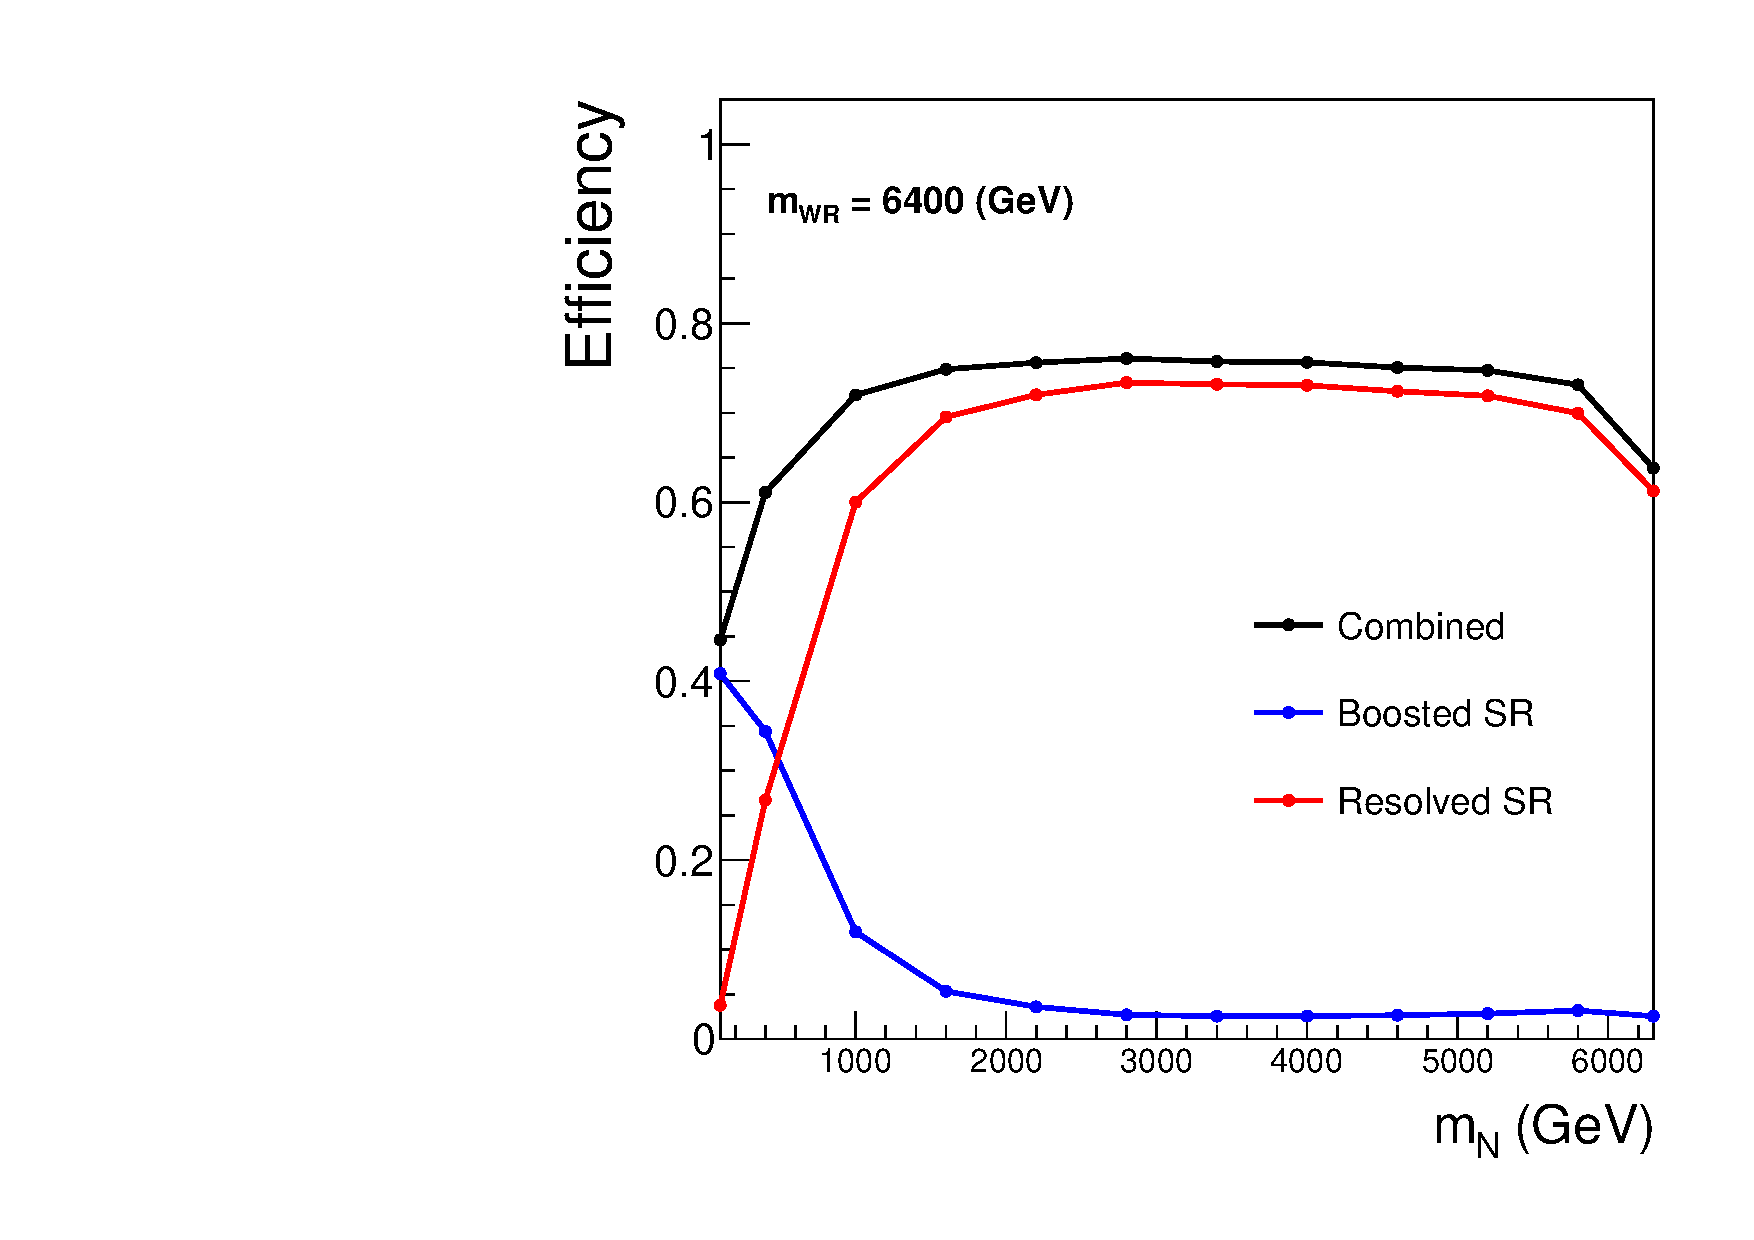
\includegraphics[width=0.45\textwidth]{figures/SigEff/WR6400.pdf}
  \hspace{0.01\textwidth}
  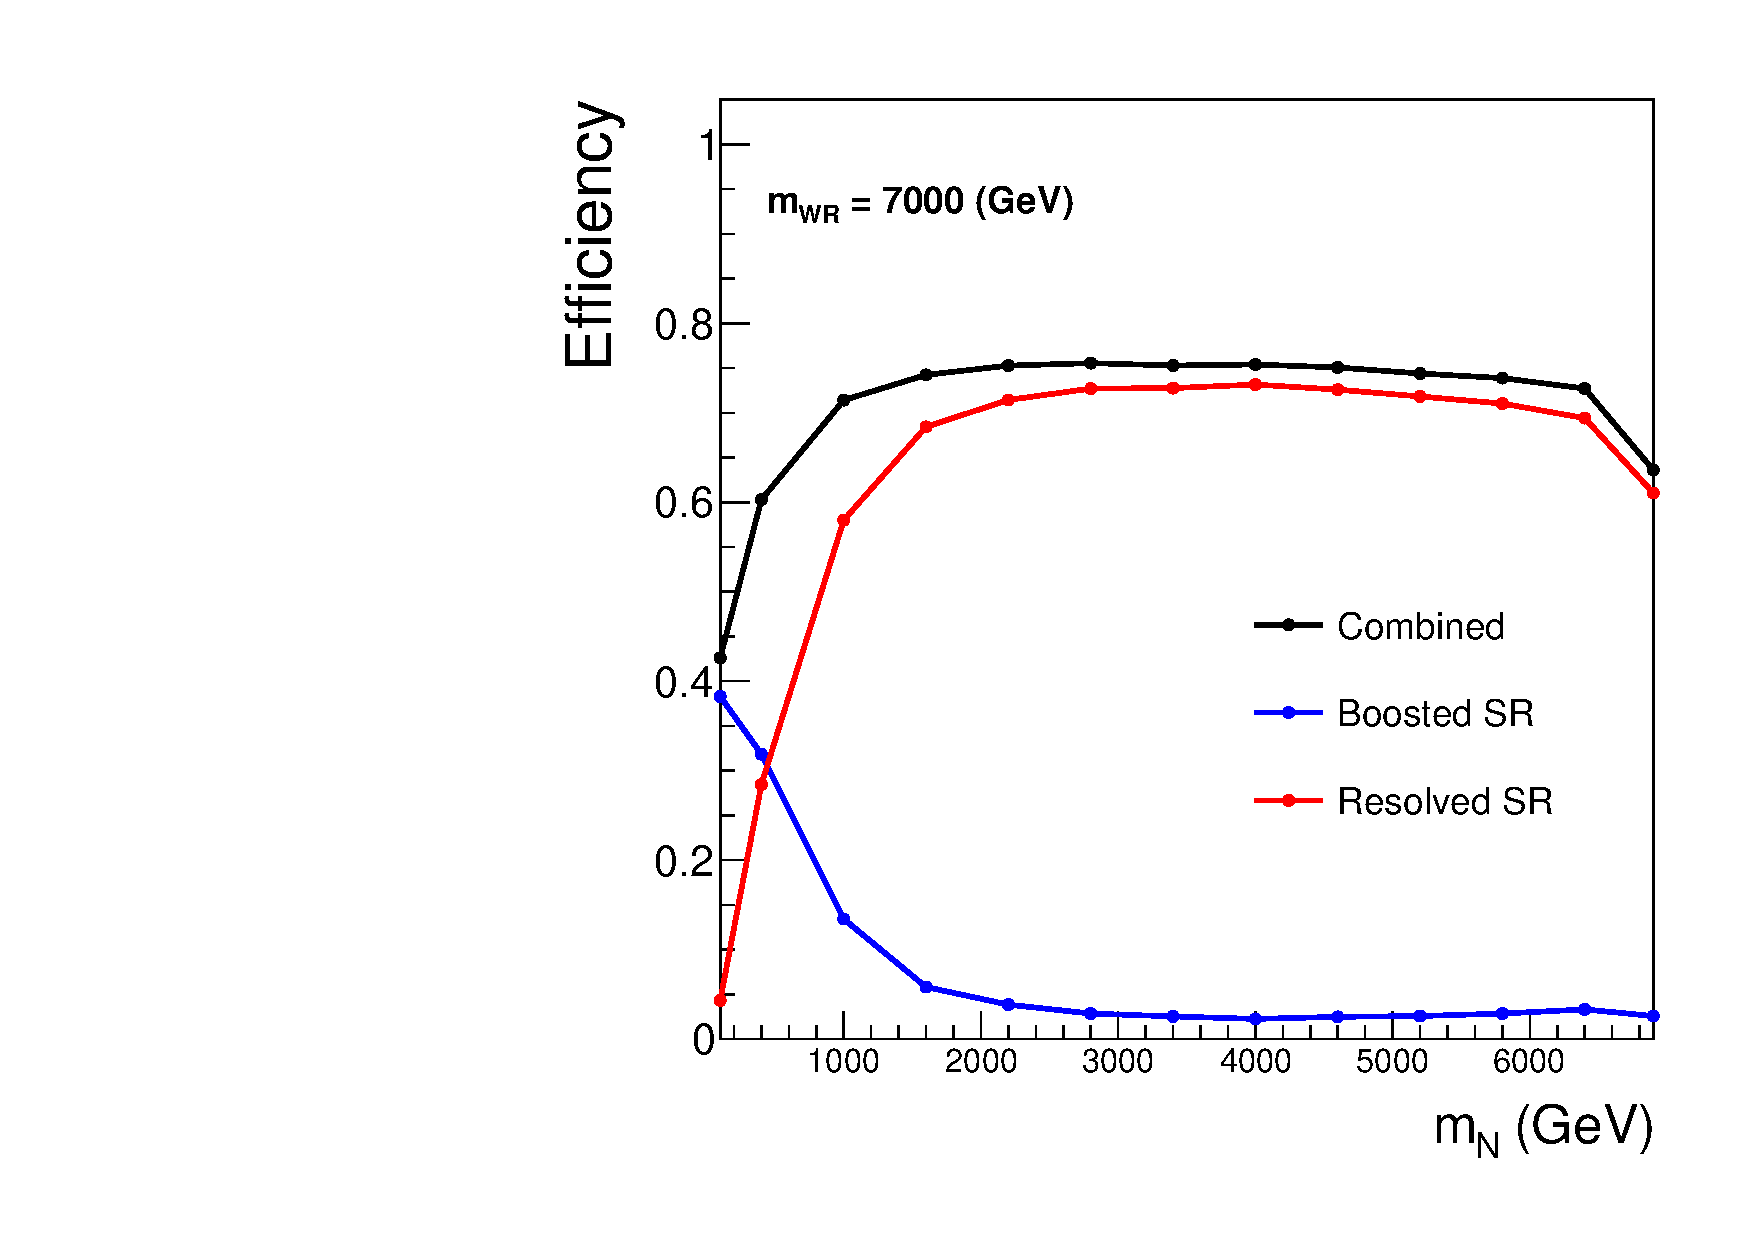
\includegraphics[width=0.45\textwidth]{figures/SigEff/WR7000.pdf}

  \caption{
    The signal efficiencies at the signal regions.
  }
  \label{fig:SigEff2}
\end{figure}

The reconstructed mass distributions of $W_{R}$ for the boosted and resolved signal regions is shown in Fig~\ref{fig:BoostedSR} and~\ref{fig:ResolvedSR}, respectively.

\subsection{Signal efficiencies}
The signal efficiencies at the signal regions are shown in Fig.~\ref{fig:SigEff1}--\ref{fig:SigEff2},
as a function $m_{N}$, for each $m_{\WR}$.







%%%%%%%%%%%%%%%%%%%%%%%%%%%%%%%%%%%%%%%%%%%%%%%%%%%%%%%%%%%%%%%%%%%%%%%%%%%%%%%%

%%%%%%%%%%%%%%%%%%%%%%%%%%%%%%%%%%%%%%%%%%%%%%%%%%%%%%%%%%%%%%%%%%%%%%%%%%%%%%%%
